%  A simple AAU report template.
%  2013-03-06 v. 1.0.0
%  Copyright 2010-2013 by Jesper Kjær Nielsen <jkn@es.aau.dk>
%
%  This is free software: you can redistribute it and/or modify
%  it under the terms of the GNU General Public License as published by
%  the Free Software Foundation, either version 3 of the License, or
%  (at your option) any later version.
%
%  This is distributed in the hope that it will be useful,
%  but WITHOUT ANY WARRANTY; without even the implied warranty of
%  MERCHANTABILITY or FITNESS FOR A PARTICULAR PURPOSE.  See the
%  GNU General Public License for more details.
%
%  You can find the GNU General Public License at <http://www.gnu.org/licenses/>.
%
\documentclass[12pt,twoside,a4paper]{report}
%%%%%%%%%%%%%%%%%%%%%%%%%%%%%%%%%%%%%%%%%%%%%%%%
% Language, Encoding and Fonts
% http://en.wikibooks.org/wiki/LaTeX/Internationalization
%%%%%%%%%%%%%%%%%%%%%%%%%%%%%%%%%%%%%%%%%%%%%%%%
% Select encoding of your inputs. Depends on
% your operating system and its default input
% encoding. Typically, you should use
%   Linux  : utf8 (most modern Linux distributions)
%            latin1 
%   Windows: ansinew
%            latin1 (works in most cases)
%   Mac    : applemac
% Notice that you can manually change the input
% encoding of your files by selecting "save as"
% an select the desired input encoding. 
%\usepackage[utf8x]{inputenc}
\usepackage[utf8]{inputenc}
% Make latex understand and use the typographic
% rules of the language used in the document.
\usepackage[danish,english]{babel}
% Use the vector font Latin Modern which is going
% to be the default font in latex in the future.
\usepackage{lmodern}
\usepackage{lastpage}
% Choose the font encoding
\usepackage[T1]{fontenc}
%%%%%%%%%%%%%%%%%%%%%%%%%%%%%%%%%%%%%%%%%%%%%%%%
% Graphics and Tables
% http://en.wikibooks.org/wiki/LaTeX/Importing_Graphics
% http://en.wikibooks.org/wiki/LaTeX/Tables
% http://en.wikibooks.org/wiki/LaTeX/Colors
%%%%%%%%%%%%%%%%%%%%%%%%%%%%%%%%%%%%%%%%%%%%%%%%
% load a colour package
\usepackage{xcolor}
\definecolor{aaublue}{RGB}{33,26,82}% dark blue
% The standard graphics inclusion package
\usepackage{graphicx}
% Trying to use this package put to replace the logo 
% with an eps vector image
\usepackage[outdir=./images/]{epstopdf}
% Set up how figure and table captions are displayed
\usepackage{caption}
\usepackage{subcaption}
\usepackage{float}
\usepackage{multirow}
\captionsetup{%
  font=footnotesize,% set font size to footnotesize
  labelfont=bf % bold label (e.g., Figure 3.2) font
}
% Make the standard latex tables look so much better
\usepackage{array,booktabs}
% Enable the use of frames around, e.g., theorems
% The framed package is used in the example environment
\usepackage{framed}
\usepackage{gensymb}

%%%%%%%%%%%%%%%%%%%%%%%%%%%%%%%%%%%%%%%%%%%%%%%%
% Mathematics
% http://en.wikibooks.org/wiki/LaTeX/Mathematics
%%%%%%%%%%%%%%%%%%%%%%%%%%%%%%%%%%%%%%%%%%%%%%%%
% Defines new environments such as equation,
% align and split 
\usepackage{amsmath}
% Adds new math symbols
\usepackage{amssymb}
% Use theorems in your document
% The ntheorem package is also used for the example environment
% When using thmmarks, amsmath must be an option as well. Otherwise \eqref doesn't work anymore.
\usepackage[framed,amsmath,thmmarks]{ntheorem}
% Emil added this for psuedo code
\usepackage{algorithm}
\usepackage{algorithmic}

\usepackage{listings}
\usepackage{color}

\definecolor{mygreen}{rgb}{0,0.6,0}
\definecolor{mygray}{rgb}{0.5,0.5,0.5}
\definecolor{mymauve}{rgb}{0.58,0,0.82}

\lstset{ %
  backgroundcolor=\color{white},   % choose the background color; you must add \usepackage{color} or \usepackage{xcolor}
  basicstyle=\footnotesize,        % the size of the fonts that are used for the code
  breakatwhitespace=false,         % sets if automatic breaks should only happen at whitespace
  breaklines=true,                 % sets automatic line breaking
  captionpos=b,                    % sets the caption-position to bottom
  commentstyle=\color{mygreen},    % comment style
  deletekeywords={...},            % if you want to delete keywords from the given language
  escapeinside={\%*}{*)},          % if you want to add LaTeX within your code
  extendedchars=true,              % lets you use non-ASCII characters; for 8-bits encodings only, does not work with UTF-8
  frame=single,                    % adds a frame around the code
  keepspaces=true,                 % keeps spaces in text, useful for keeping indentation of code (possibly needs columns=flexible)
  keywordstyle=\color{blue},       % keyword style
  language=C++,                 % the language of the code
  morekeywords={*,...},            % if you want to add more keywords to the set
  numbers=left,                    % where to put the line-numbers; possible values are (none, left, right)
  numbersep=5pt,                   % how far the line-numbers are from the code
  numberstyle=\tiny\color{mygray}, % the style that is used for the line-numbers
  rulecolor=\color{black},         % if not set, the frame-color may be changed on line-breaks within not-black text (e.g. comments (green here))
  showspaces=false,                % show spaces everywhere adding particular underscores; it overrides 'showstringspaces'
  showstringspaces=false,          % underline spaces within strings only
  showtabs=false,                  % show tabs within strings adding particular underscores
  stepnumber=1,                    % the step between two line-numbers. If it's 1, each line will be numbered
  stringstyle=\color{mymauve},     % string literal style
  tabsize=2,                       % sets default tabsize to 2 spaces
  title=\lstname                   % show the filename of files included with \lstinputlisting; also try caption instead of title
}

%%%%%%%%%%%%%%%%%%%%%%%%%%%%%%%%%%%%%%%%%%%%%%%%
% Page Layout
% http://en.wikibooks.org/wiki/LaTeX/Page_Layout
%%%%%%%%%%%%%%%%%%%%%%%%%%%%%%%%%%%%%%%%%%%%%%%%
% Change margins, papersize, etc of the document
\usepackage[margin=3cm]{geometry}
% Modify how \chapter, \section, etc. look
% The titlesec package is very configureable
\usepackage{titlesec}
\titleformat*{\section}{\normalfont\Large\bfseries\color{aaublue}}
\titleformat*{\subsection}{\normalfont\large\bfseries\color{aaublue}}
\titleformat*{\subsubsection}{\normalfont\normalsize\bfseries\color{aaublue}}
%\titleformat*{\paragraph}{\normalfont\normalsize\bfseries\color{aaublue}}
%\titleformat*{\subparagraph}{\normalfont\normalsize\bfseries\color{aaublue}}
\usepackage{parskip}% http://ctan.org/pkg/parskip
\setlength{\parindent}{0pt}


% Change the headers and footers
\usepackage{fancyhdr}
\pagestyle{fancy}
\fancyhf{} %delete everything
\renewcommand{\headrulewidth}{0pt} %remove the horizontal line in the header
\fancyhead[RE]{\color{aaublue}\small\nouppercase\leftmark} %even page - chapter title
\fancyhead[LO]{\color{aaublue}\small\nouppercase\rightmark} %uneven page - section title
\fancyhead[LE,RO]{\thepage} %page number on all pages
% Do not stretch the content of a page. Instead,
% insert white space at the bottom of the page
\raggedbottom
% Enable arithmetics with length. Useful when
% typesetting the layout.
\usepackage{calc}

%%%%%%%%%%%%%%%%%%%%%%%%%%%%%%%%%%%%%%%%%%%%%%%%
% Bibliography
% http://en.wikibooks.org/wiki/LaTeX/Bibliography_Management
%%%%%%%%%%%%%%%%%%%%%%%%%%%%%%%%%%%%%%%%%%%%%%%%
% Add the \citep{key} command which display a
% reference as [author, year]
\usepackage{cite}
\usepackage{notoccite}
%\usepackage[square]{natbib}
% Appearance of the bibliography
%\bibliographystyle{apalike}

%%%%%%%%%%%%%%%%%%%%%%%%%%%%%%%%%%%%%%%%%%%%%%%%
% Misc
%%%%%%%%%%%%%%%%%%%%%%%%%%%%%%%%%%%%%%%%%%%%%%%%
% Add bibliography and index to the table of
% contents
\usepackage[nottoc]{tocbibind}
% Add the command \pageref{LastPage} which refers to the
% page number of the last page
\usepackage[
%  disable, %turn off todonotes
  colorinlistoftodos, %enable a coloured square in the list of todos
  textwidth=\marginparwidth, %set the width of the todonotes
  textsize=scriptsize, %size of the text in the todonotes
  ]{todonotes}

%%%%%%%%%%%%%%%%%%%%%%%%%%%%%%%%%%%%%%%%%%%%%%%%
% Hyperlinks
% http://en.wikibooks.org/wiki/LaTeX/Hyperlinks
%%%%%%%%%%%%%%%%%%%%%%%%%%%%%%%%%%%%%%%%%%%%%%%%
% Enable hyperlinks and insert info into the pdf
% file. Hypperref should be loaded as one of the 
% last packages
\usepackage{hyperref}
\hypersetup{%
	plainpages=false,%
	pdfauthor={Author(s)},%
	pdftitle={Title},%
	pdfsubject={Subject},%
	bookmarksnumbered=true,%
	colorlinks,%
	citecolor=aaublue,%
	filecolor=aaublue,%
	linkcolor=aaublue,%
	urlcolor=aaublue,%
	pdfstartview=FitH%
}

%%%%%%%%%%%%%%%%%%%%%%%%%%%%%%%%%%%%%%%%%%%%%%%%%%%%%%%%%%
% Listings
% http://en.wikibooks.org/wiki/LaTeX/Source_Code_Listings
%%%%%%%%%%%%%%%%%%%%%%%%%%%%%%%%%%%%%%%%%%%%%%%%%%%%%%%%%%
% Using the package listings you can add non-formatted text 
% as you would do with \begin{verbatim} but its main aim is 
% to include the source code of any programming language within 
% your document. If you wish to include pseudocode or algorithms, 
% you may find Algorithms and Pseudocode useful also.
\usepackage{listings}
\usepackage{color}

\definecolor{dkgreen}{rgb}{0,0.6,0}
\definecolor{gray}{rgb}{0.5,0.5,0.5}
\definecolor{mauve}{rgb}{0.58,0,0.82}

\lstset{frame=tb,
	language=Java,
	aboveskip=3mm,
	belowskip=3mm,
	showstringspaces=false,
	columns=flexible,
	basicstyle={\small\ttfamily},
	numbers=none,
	numberstyle=\tiny\color{gray},
	keywordstyle=\color{blue},
	commentstyle=\color{dkgreen},
	stringstyle=\color{mauve},
	breaklines=true,
	breakatwhitespace=true,
	tabsize=3
}

\input{setup/Hyphenations.tex}
\input{setup/Macros.tex}

\begin{document}
\sloppy
\pagenumbering{roman}

\newcommand{\HRule}{\rule{\linewidth}{0.5 mm}}
\begin{titlepage}

\begin{center}
% Upper part of the page
\iflanguage{danish}{%
	\includegraphics[width=0.6\textwidth]{images/aau_logo_de}
}{%
	
\includegraphics[width=0.6\textwidth]{images/aau_logo_en}
}\\[0.5cm]

\textsc{\Large ED2 - P2 - H103}\\[0.6cm]

% Title
\HRule \\[0.9cm]
{ \Huge \bfseries Mapping and navigation of unknown terrain }\\[0.4cm]

\HRule \\[0.5cm]


% Author and supervisor
\begin{minipage}{0.49\textwidth}
\begin{flushleft} \large
\emph{Students:}\\
Antal János Monori\\
Emil Már Einarsson\\
Gustavo Smidth Buschle\\
Thomas Thuesen Enevoldsen
\end{flushleft}
\end{minipage}
\begin{minipage}{0.49\textwidth}
\begin{flushright} \large
\emph{Supervisor:} \\
Akbar Hussain\\
Torben Rosenørn
\end{flushright}
\end{minipage}

\vfill

% Bottom of the page
{\large \today}



\end{center}

\end{titlepage}
\cleardoublepage
\pdfbookmark[0]{English title page}{label:titlepage_en}
\aautitlepage{%
  \englishprojectinfo{
    P2 preliminary title
  }{%
    Scientific Theme %theme
  }{%
    Spring Semester 2015 %project period
  }{%
    H103 % project group
  }{%
    %list of group members
	Antal János Monori\\
	Emil Már Einarsson\\
	Gustavo Smidth Buschle\\
	Michal Damian Budzinski\\
	Thomas Thuesen Enevoldsen
  }{%
    %list of supervisors
	Akbar Hussain\\
	Torben Rosenørn
  }{%
    1 % number of printed copies
  }{%
    \today % date of completion
  }%
}{%department and address
  \textbf{School of Information and Communication Technology}\\
  Niels Bohrs Vej 8\\
  DK-6700 Esbjerg\\
  \href{http://sict.aau.dk}{http://sict.aau.dk}
}{% the abstract
	Abstract
}
\date{\today}
\cleardoublepage

\tableofcontents

\cleardoublepage


\chapter*{Preface\markboth{Preface}{Preface}}\label{ch:preface}
\addcontentsline{toc}{chapter}{Preface}

%TODO: P2 project preface

From hereby on, every mention of 'we' refers to the four co-authors listed below.


\vspace{\baselineskip}\hfill Aalborg University, \today
\vfill\noindent
\begin{minipage}[b]{0.45\textwidth}
	\centering
	\rule{\textwidth}{0.5pt}\\
	Antal János Monori\\
	{\footnotesize <amonor14@student.aau.dk>}
\end{minipage}
\hfill
\begin{minipage}[b]{0.45\textwidth}
	\centering
	\rule{\textwidth}{0.5pt}\\
	Emil Már Einarsson\\
	{\footnotesize <eeinar14@student.aau.dk>}
\end{minipage}
\vspace{3\baselineskip}

\vspace{5mm}\noindent 
\begin{minipage}[b]{0.45\textwidth}
	\centering
	\rule{\textwidth}{0.5pt}\\
	Gustavo Smidth Buschle\\
	{\footnotesize <gbusch14@student.aau.dk>}
\end{minipage}
\hfill
\begin{minipage}[b]{0.45\textwidth}
	\centering
	\rule{\textwidth}{0.5pt}\\
	Thomas Thuesen Enevoldsen\\
	{\footnotesize <tten14@student.aau.dk>}
\end{minipage}
\vspace*{3\baselineskip}


\pagenumbering{arabic}
%Chapter 1  ------------
\chapter{Introduction}\label{ch:introduction}

We started out the project with a brainstorming session where we discussed different problems we would like to solve. By the end of the session, we came up with the following list of problems:
\begin{itemize}
	\item Noise pollution
	\item Navigation using echolocation
	\item Re-usability of heat waste
	\item Mapping of unknown terrains without any external technologies
	\item Maze navigation
\end{itemize}

We could identify a common theme amongst these problems, which led us to the conclusion that the problem-domain should be within mapping and navigation. 

\begin{figure}[!h]
	\centering
	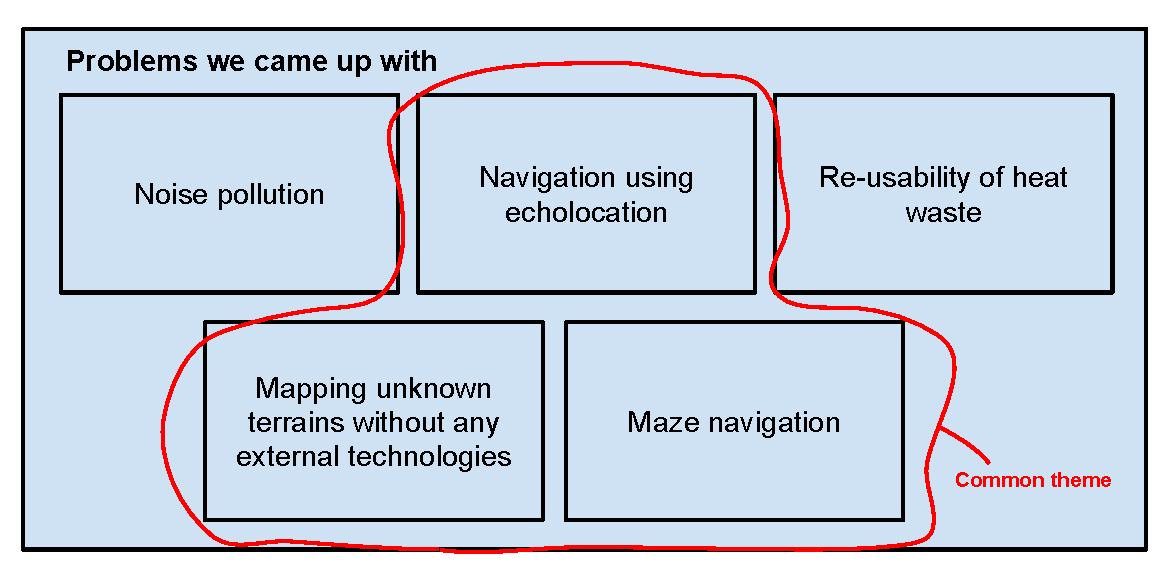
\includegraphics[scale=.7]{images/high-level-block.pdf}
	\caption{High-level block diagram expanding upon our brainstorming session}
	\label{fig:highlevelblock}
\end{figure}

Furthermore we decided to expand upon the problem-domain we set for ourselves and to further explore it. This led to more discussions on possible outcomes, implementations and benefits of such system.

\begin{figure}[!h]
	\centering
	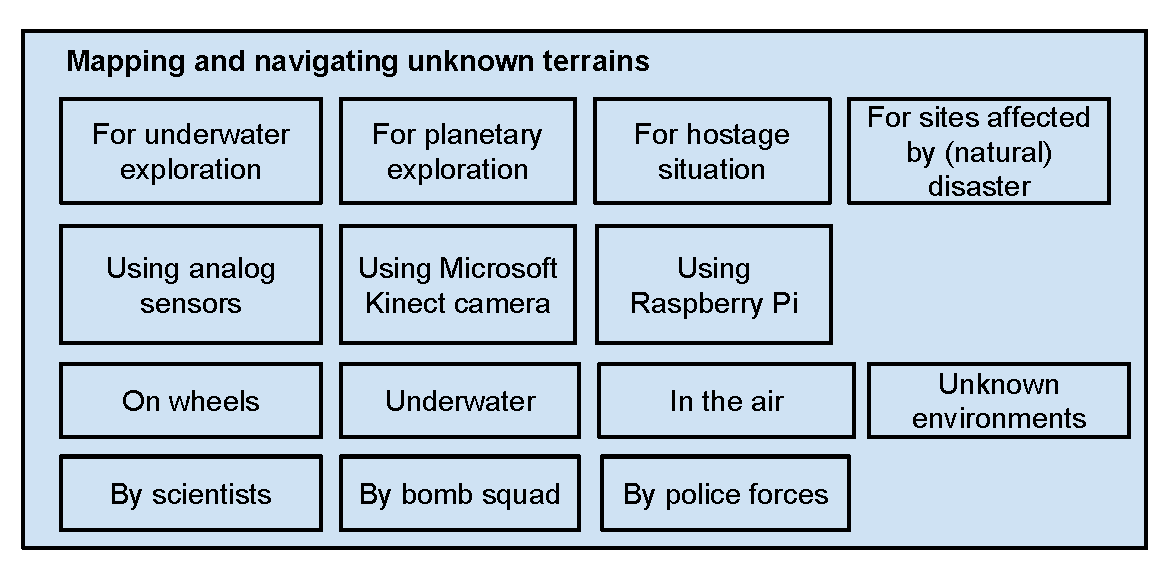
\includegraphics[scale=.7]{images/low-level-block.pdf}
	\caption{Low-level block diagram expanding upon the common theme we found}
	\label{fig:lowlevelblock}
\end{figure}

We decided to continue on with the selected problem-domain and started using a W-diagram model to expand upon it further and to identify the parts needed to be researched. This method will help us to come up with a solution to the problem at hand.

\section{Initiating Problem}
The initiating problem selected is \textit{unknown terrain mapping and navigation}.

%Chapter 2  ------------
\chapter{Problem Analysis}\label{ch:problem_analysis}

Since the beginning of time, early human settlements were eager to explore their environment and surroundings. It did not take long, until the first humans started getting even further and become explorers. They started leaving marks and using landmarks to remember pathways and places. This primitive representation of prehistoric places and early history maps can be traced back to 24000-25000 BC\cite{cavedrawings}. Soon after, they started using maps, which revolutionized the way we navigate and the way we travel, - and therefore the field of Cartography was born. During the 19th century terra incognita (Latin, ‘unknown land.’) disappeared from maps, since both the coastlines and the inner parts of the continents had been fully explored. Today, using technology and satellites, Earth is completely mapped, yet still not completely explored. Around 95 percent of our oceans are still remains unexplored, considering that they take up 70 percent of the planet's surface\cite{oceandepth}. This is mostly due to extreme conditions and high depths, that humans can not be put up against. As technology advanced and matured, remotely operated underwater vehicles (ROVs) become a popular way of exploring the depths of our oceans, due to their accessibility to places where humans could not possibly go before for a long period of time. In the meantime, interplanetary exploration took off during the mid-20th century with the start of the Cold War between the United States of America and the Soviet Union. This led to many great achievements in the field, like the first successful interplanetary encounter, where the US Mariner 2 flew by Venus\cite{firstflyby} or when the Soviet Venera 3 made first impact on the surface of Venus\cite{firstimpact}. The last successful program to date was the Mars rover CURIOSITY, which landed and still making progress in exploring and sending back scientific data of the planet Mars. Exploring planets for future-settlements and first-contact is very important in order to quench out human curiosity but also for advancing the different fields in science and technology.

\clearpage

\begin{figure}[!h]
	\centering
	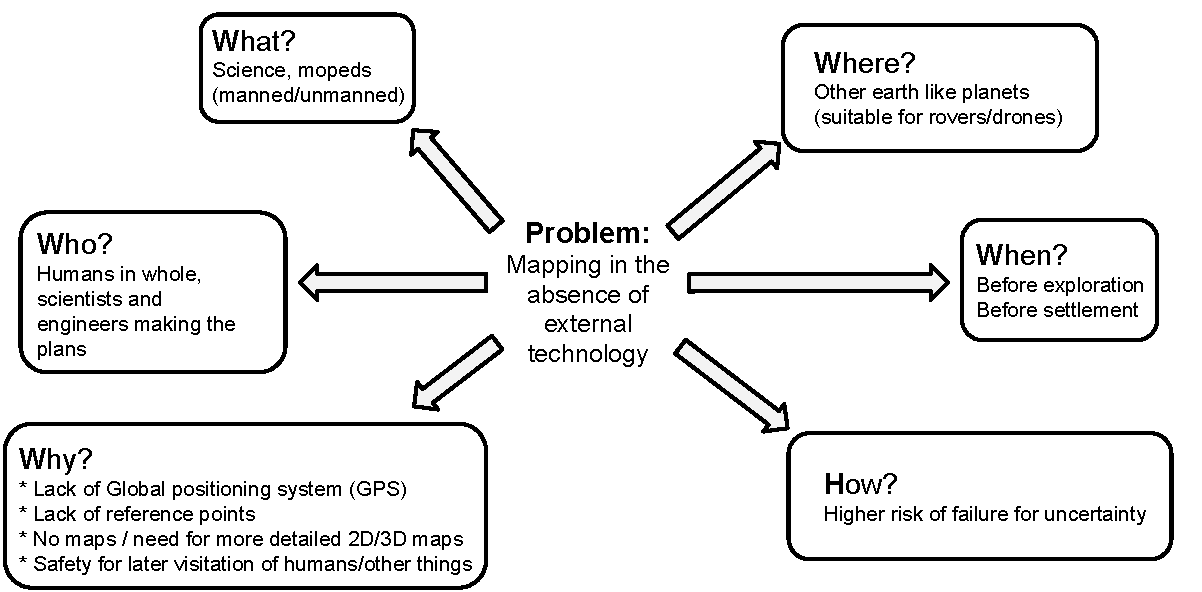
\includegraphics[scale=.7]{images/wdiagram1.pdf}
	\caption{W-diagram}
	\label{fig:wdiagram}
\end{figure}

\subsection{When is this actually a problem?}
Mapping unknown terrains becomes a problem when new planets are discovered and mapping of the surface and its atmosphere is required for further exploration and investigation. Scientists use the so-called Earth Similarity Index (ESI) for mapping extrasolar planets (also called exoplanets) for potentially habitable places in the Universe.\cite{exoplanets}\cite{esi}. The ESI implies many factors, like surface temperature and other Earth-like properties. 

Another scenario is underwater exploration, where trained divers are unable to explore and map the underwater terrain due to its depth and dangerous circumstances. In these cases robots and submarines, that can either autonomously or remote-controlled can take up the task of mapping the bottom of the ocean. It is also much faster and more reliable than sending down people to do the same task.

Besides exploration, the task of mapping unknown terrains is used in hostage situation and natural disasters as well, where people cannot enter a specific area without that being mapped upfront for various factors, like radiation leakage or armed terrorists. One example would be the Fukushima Nuclear Plant catastrophe in Fukushima, Japan on March, 2011. After the leakage in the reactor, rescue forces and scientist used autonomous drones to map the inside of the factory\cite{fukushima}, which was put under quarantine for high levels or radiation and therefore no person was allowed inside of the building without proper precautions. Drones and autonomous robots are perfect for scenarios like this.

\subsection{Where does this problem actually occur?}
Unknown terrain can be defined as a terrain where no mapping has been done before.

The bottom of the ocean is mostly sand, mud, and water [%TODO: citation needed.
]. This makes it difficult to navigate with a rover, but relatively simple to navigate with a submarine. In water, sensors that use sound need to be calibrated to work with the correct pressure of the water surrounding it, which varies with the depth of the water. If the water is murky, light based sensors may also not work, depending on the wavelength of the light they use. Light also refracts in water depending on the water density. It is possible to remote-control vehicles in the bottom of the ocean.

Other planets can be much more complicated to navigate. The consistency of they atmosphere and terrain may be not completely understood. This means that there is a higher chance of a rover being stuck on loose terrain, falling down sheer faces, and so on. It may also be the case that the planet has no atmosphere, so a drone would not be able to hover. One of the biggest issues with extraplanetary exploration is input lag. Other planets are very far away, which means that signals traveling to these distant places can take several minutes at least and years at most to reach from the Earth, thus automation is better suited for this task. Other planets share the issues that the bottom of the ocean has with sensors.

Disaster scenarios can also be said to be unknown terrain. Disaster scenarios means that the terrain might be loose or difficult to navigate, so a drone might be best suited for it. In most cases disaster scenarios happen in locations where the vehicle can be controlled manually.

\subsection{How is it a problem?}

To answer the question how does this problem occur, we have to look into some possible scenarios discussed above. Exploration of unknown terrain and environments has been practised for many years. It originates from the human curiosity and the spirit to explore and gather information about our surroundings, discussed previously.

When dealing with unknown environments, unknown does not strictly refer to the environment itself but the persons state of knowledge about the physics and composition of the given environment. In a known environment, outcomes from every action can more or less be calculated or estimated. Where as in an unknown environment, it is a matter of investigation and figuring out what works and what does not. In the unknown environment it is important to gain knowledge of how everything work, so that in the future it possible for an individual make the best possible choice and decisions in the environment.\cite{aiint}
Even though most of the land has been explored and is being used for its vast amount of resources, the time will come where planetary and ocean exploration becomes a key factor for our technological advancements and our resources. Ocean exploration is important because it provides data from deep-sea areas, which in turn will reduce the amount of unknown environments left on our planet.
Gathering data and intelligence from the ocean also helps with managing the resources that are available in the deep-sea areas, so that future generations can benefit from them. The ocean also provides information about future environmental conditions and can help predict earthquakes and tsunamis. Investigating the deep-sea also reveals new ecosystems and possible sources for medication, food and energy, which are all vital for scientific advancements.\cite{oceanexplo}

Humans have always had never-ending interest and need to push science and technology to its limits, and then desire to achieve something even further than what is possible. The many challenges humans have faced has led to many benefits for our society almost since its creation. Space exploration helps further our understanding about the history of our universe and solar system.\cite{whyweexplo}

\subsection{To whom and what is this a problem?}
Unknown terrains and environments pose a big issue for scientists and engineers who want to explore these areas. Designing vehicles and devices for the deep-sea ocean or planetary exploration is impossible, without any background information on what environmental factors they will be dealing with or encountering. Exploration is essential when in the future new resources are needed for scientific and technological advancements, that currently our of reach.

In the long run humans in general will be affected by the lack of exploration. Alternative resources and habitable areas for expansion will be necessary in the future, when earth's natural resource deposits become depleted and there are less habitable places. 

Scientists are heavily hindered by society, because it is becoming too focused on risks. Only 5 percent of the ocean has been explored, this leaves a large amount of areas untouched and mapped. Being concerned about taking risks is what will put the future development and science in jeopardy.\cite{risksandexplo} 

\subsection{Why is this a problem?}
The reason why we need to explore other unknown terrains is to help us better understand everything around us and to be able to go to other planets. 
%TODO: What? // If we are flying in the dark about the terrain underwater or on another planet and we are planning of settling there or use those resources then we have a bigger change of failure. 
If the trips are planned well and we make a good 3D map of the terrain we can come up with better plans on the next mission or if we want to use this location at all. 

The problems with navigating a robot in an unknown terrain is the lack of reference points that are needed to make a 3D map and also reference point for the robot itself to being able to navigate. That makes two challenges for us. One is for the robot to being able to navigate through a completely unknown terrain and at the same time make sense of it and come up with reference point that will be use to make a 3D map.

If a robot is successful with that task and we get back a detailed 3D map then the next mission can rely on that information and have a easier way to navigate. 

On Earth, we have the GPS (global positioning system) that is a space-based satellite navigation system flying over the Earth\cite{gpsgeneral}. Putting up a system like that on another planet cost a lot of resources and the cost to start with would not be beneficial in the beginning. GPS also does not penetrate water\cite{underwatergps}. 

\clearpage
\section{Autonomous Vehicles and Robots}

Autonomous robots or vehicles can work for an extended period of time gathering information from its surroundings to be able to work without human intervention. The robot or vehicles gathers different kinds of data, depending on what the goal of the robot it.Positional data can be utilized for navigation and path finding in a known and unknown environment. Intelligent autonomous devices are able to adapt to changes happening in its surroundings.
Currently there are many robots on the market that are self-reliant, ranging from autonomous vacuum cleaner to drones and helicopters. \cite{autonomousbasic}

Simple autonomous robots use ultrasonic sensors or infrared to manipulate itself if it detects obstacles. The is useful for obstacle avoidance and mapping of unknown areas, where the robot through a reference point can pin-point the obstacles it has encountered along the way.
More advanced robots use vision to grant them the ability to see their surroundings, algorithms analyse the camera data and gives the robot depth perception, which grants the robot the ability to instantly identify objects and locate them immediately.\cite{obstacles}

There exists two kinds of autonomous robots, a single computer autonomous robot and insect robots. The single computer autonomous robot uses its own on-board computing unit to do its computations and decisions, whereas the the insect robots are a fleet a many robots who are controlled by a single separate computing unit.
The advantage of having a single computer autonomous robot is that the tasks it performs can be done using more computer resources. It has the possibility of utilizing the computing power to its full potential, instead of relying on a separate unit that is also making decisions and calculations for many other robots.
The individual robot in the insect family is simple, but the whole robot fleet can be advanced and possibly perform sophisticated tasks, that a require multiple simpler robots.\cite{singleandinsect}



\section{Path finding and mapping}

Pathfinding is done by a computer, where it uses plotting to find the shortest path between two different points. It can be viewed as a more efficient way of navigating a maze.
There exists pathfinding algorithms that are used for software simulations, but also for mobile robot navigation. 

A common pathfinding algorithm is A* (A star) and its extended version D*.
%Needs some more transitioning information

The A* algorithm is most commonly used in video games. The algorithm determines that cost of steps per movement(\textbf{G}) in relation to the estimated cost  of steps towards its destination (\textbf{H}). Possible paths surrounding the current position are analysed and the path with the lowest sum(\textbf{F}) of the step cost and the estimated step cost is the chosen path.\cite{astar}
%maybe add one of the block images from (good source on A*) http://www.policyalmanac.org/games/aStarTutorial.htm
%Intro to A* http://www.raywenderlich.com/4946/introduction-to-a-pathfinding
%Possible more A* information http://heyes-jones.com/astar.php
%Robots using A*? http://www.pdx.edu/computer-science/sites/www.pdx.edu.computer-science/files/TR%2012-02.pdf
%Robots using A* for navigation? http://ais.informatik.uni-freiburg.de/publications/papers/thesis_bennewitz.pdf


D*, the extended version of A*
%Information regarding D*
%http://www.frc.ri.cmu.edu/~axs/dynamic_plan.html
%http://www.frc.ri.cmu.edu/~axs/doc/icra94.pdf
%http://idm-lab.org/project-a.html


Line tracking
%http://www.ikalogic.com/line-tracking-sensors-and-algorithms/

Motion and sound
%http://www.seas.upenn.edu/sunfest/docs/slides/HuangLouie05.pdf
%http://www.extremetech.com/extreme/159347-pathfinding-is-the-key-to-putting-robot-pack-mules-in-the-field
%http://5drobotics.com/
%http://www.kuka-labs.com/en/service_robotics/mobile_robotics/autonomous_navigation/

%Advanced imagery stufferino
%http://ilab.usc.edu/publications/doc/Siagian_etal13icra.pdf

%Misc
%http://www.doc.ic.ac.uk/~nd/surprise_97/journal/vol4/jmd/
%http://www.doc.ic.ac.uk/~nd/surprise_97/journal/vol1/jmd/




%Chapter 3  ------------
\clearpage
\chapter{Problem Definition}\label{ch:problem_definition}

%\section{Conclusion of Problem Analysis}

During the research for this project, we have figured out what technologies we will use when solving our problem, that is stated in the W-diagram.
We will be using a rover to navigate around with multiple sensors. Making a 2D map of its surroundings, with the possibility of implementing equipment for 3D mapping. We will be using both sound and light sensors for navigation and mapping. Ultrasonic-sensors will be used for close encounter maneuvers for their high precision at a close range (up to 4m)\cite{ultra}. For mapping we will be using a laser sensor, that will either automatically turn 360$^{\circ}$  or we will implement a motor to rotate the sensor.
The rover will both be remote controlled and autonomous for navigation. For reference points we will be using the ultrasonic-sensors. The control computer will be a Raspberry Pi running a Debian Unix operating system. The reason for using the Raspberry Pi is that it can multi-task, read many sensors at the same time and build the 2D map on the go. For other microcontrollers, like the Arduino, we would only be able to collect data and need to build the map from it later, using another computer. 

\begin{figure}[H]
	\centering
	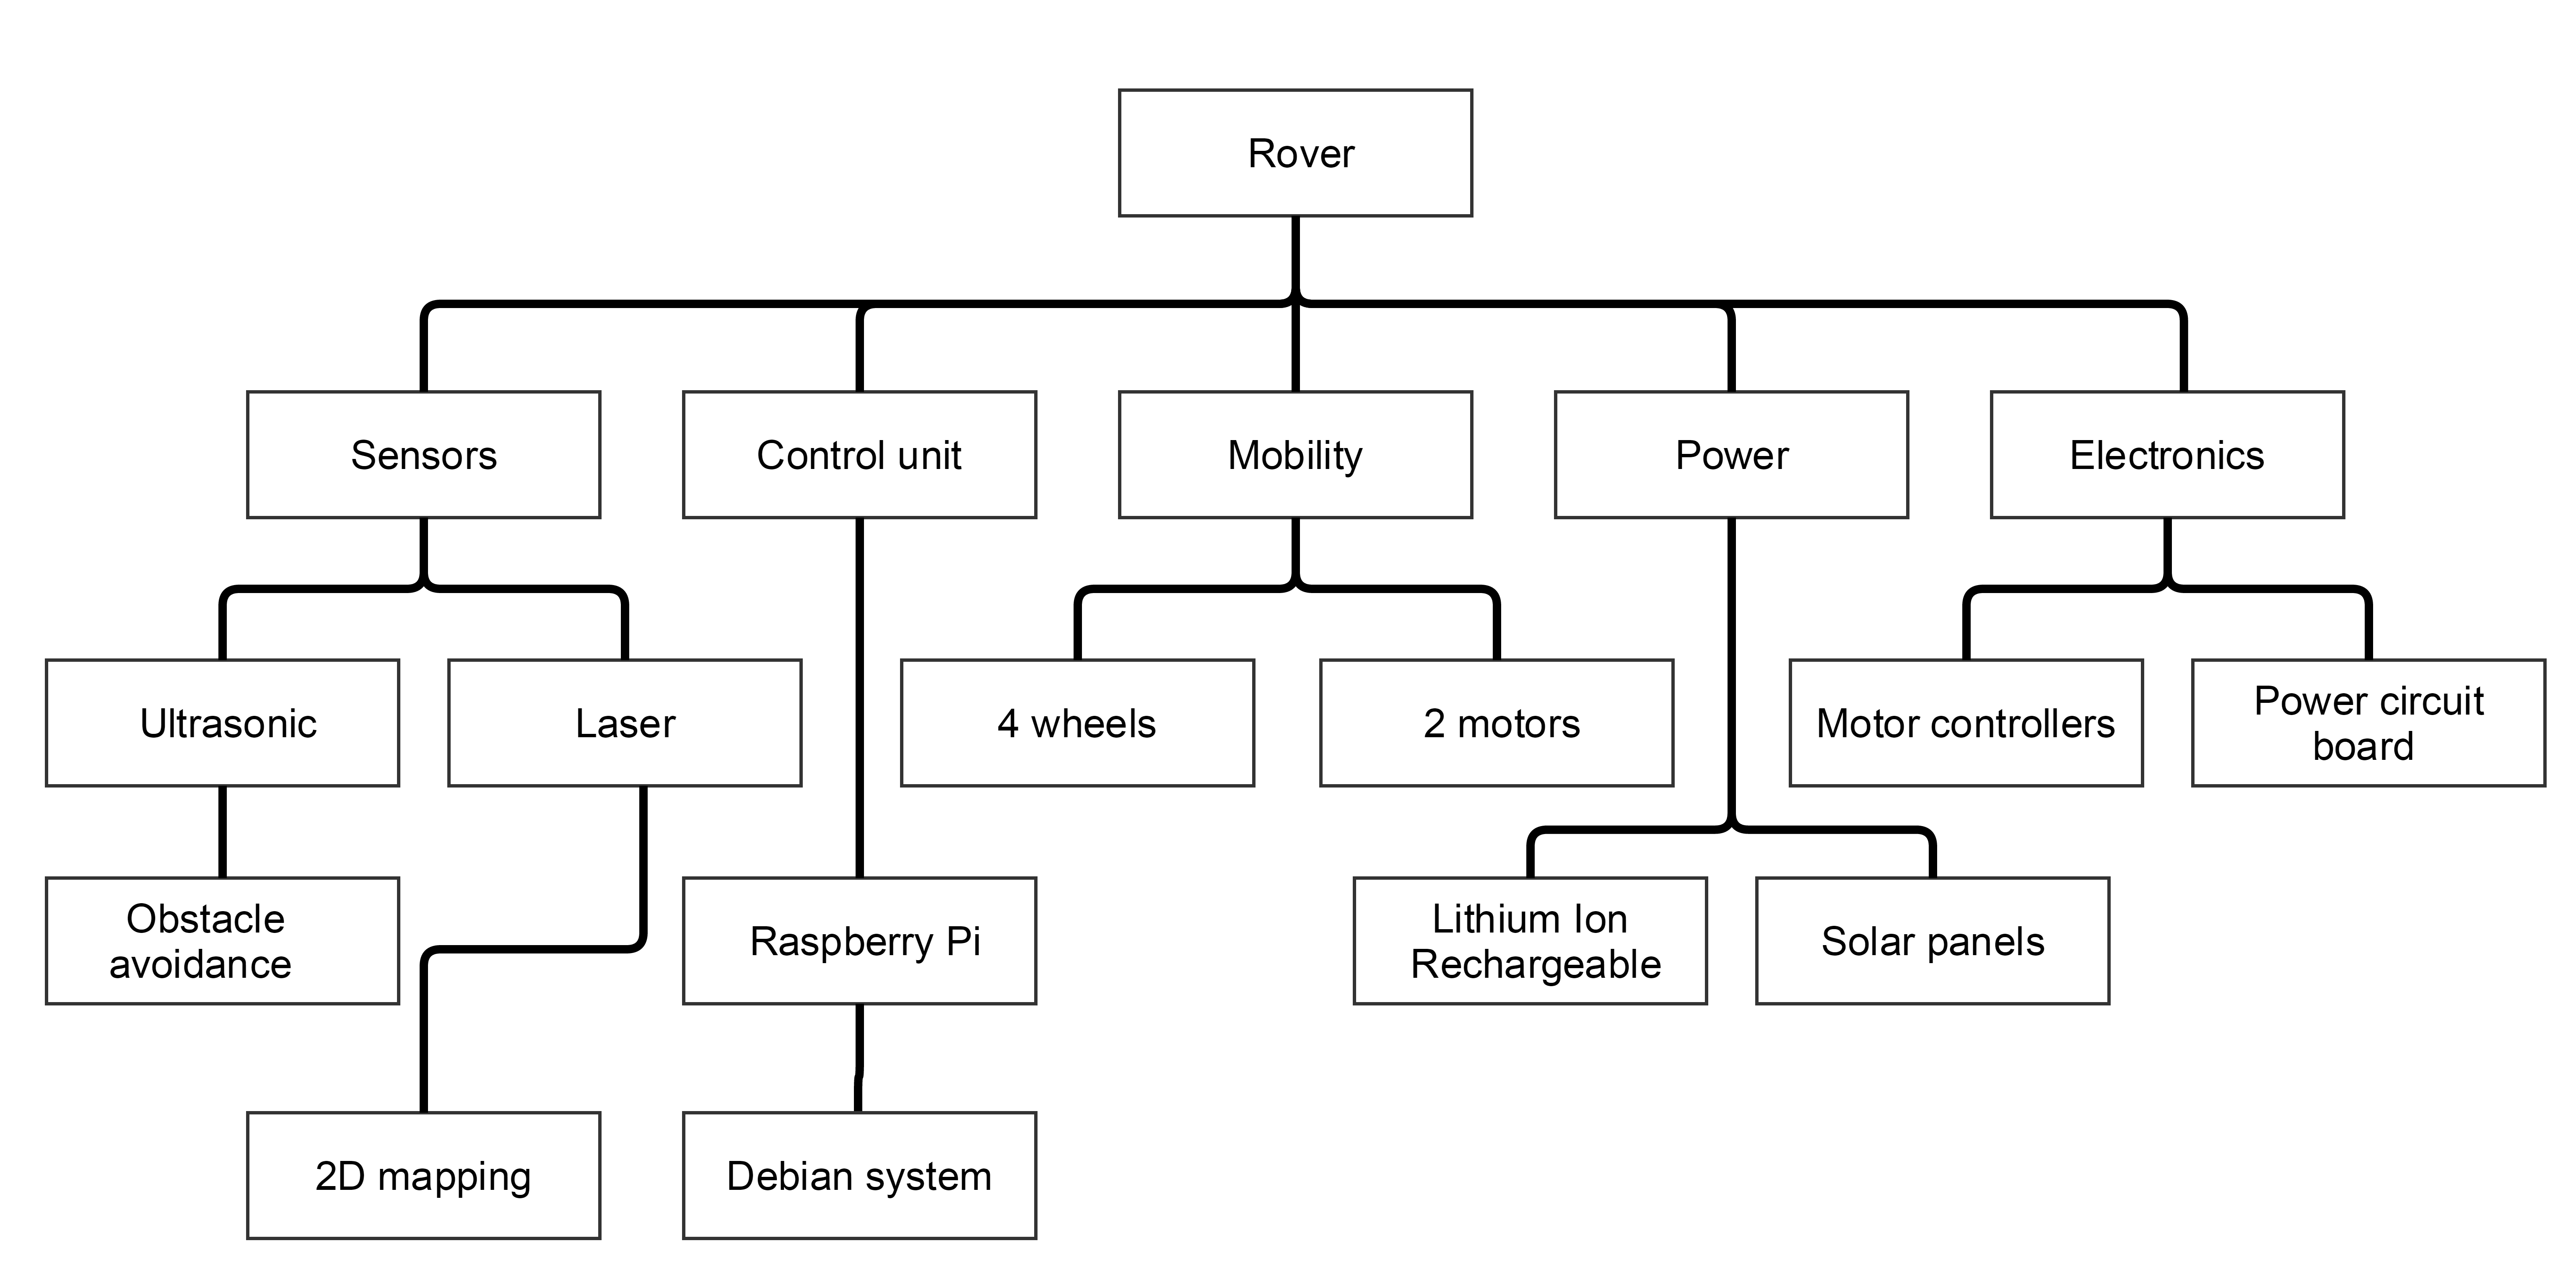
\includegraphics[scale=.1]{images/level2.png}
	\caption{Flowchart of the prototype idea.}
	\label{fig:level2}
\end{figure}

On this flowchart you can see how we expend from the level 1 flowchart in chapter 1.

\begin{figure}[H]
	\centering
	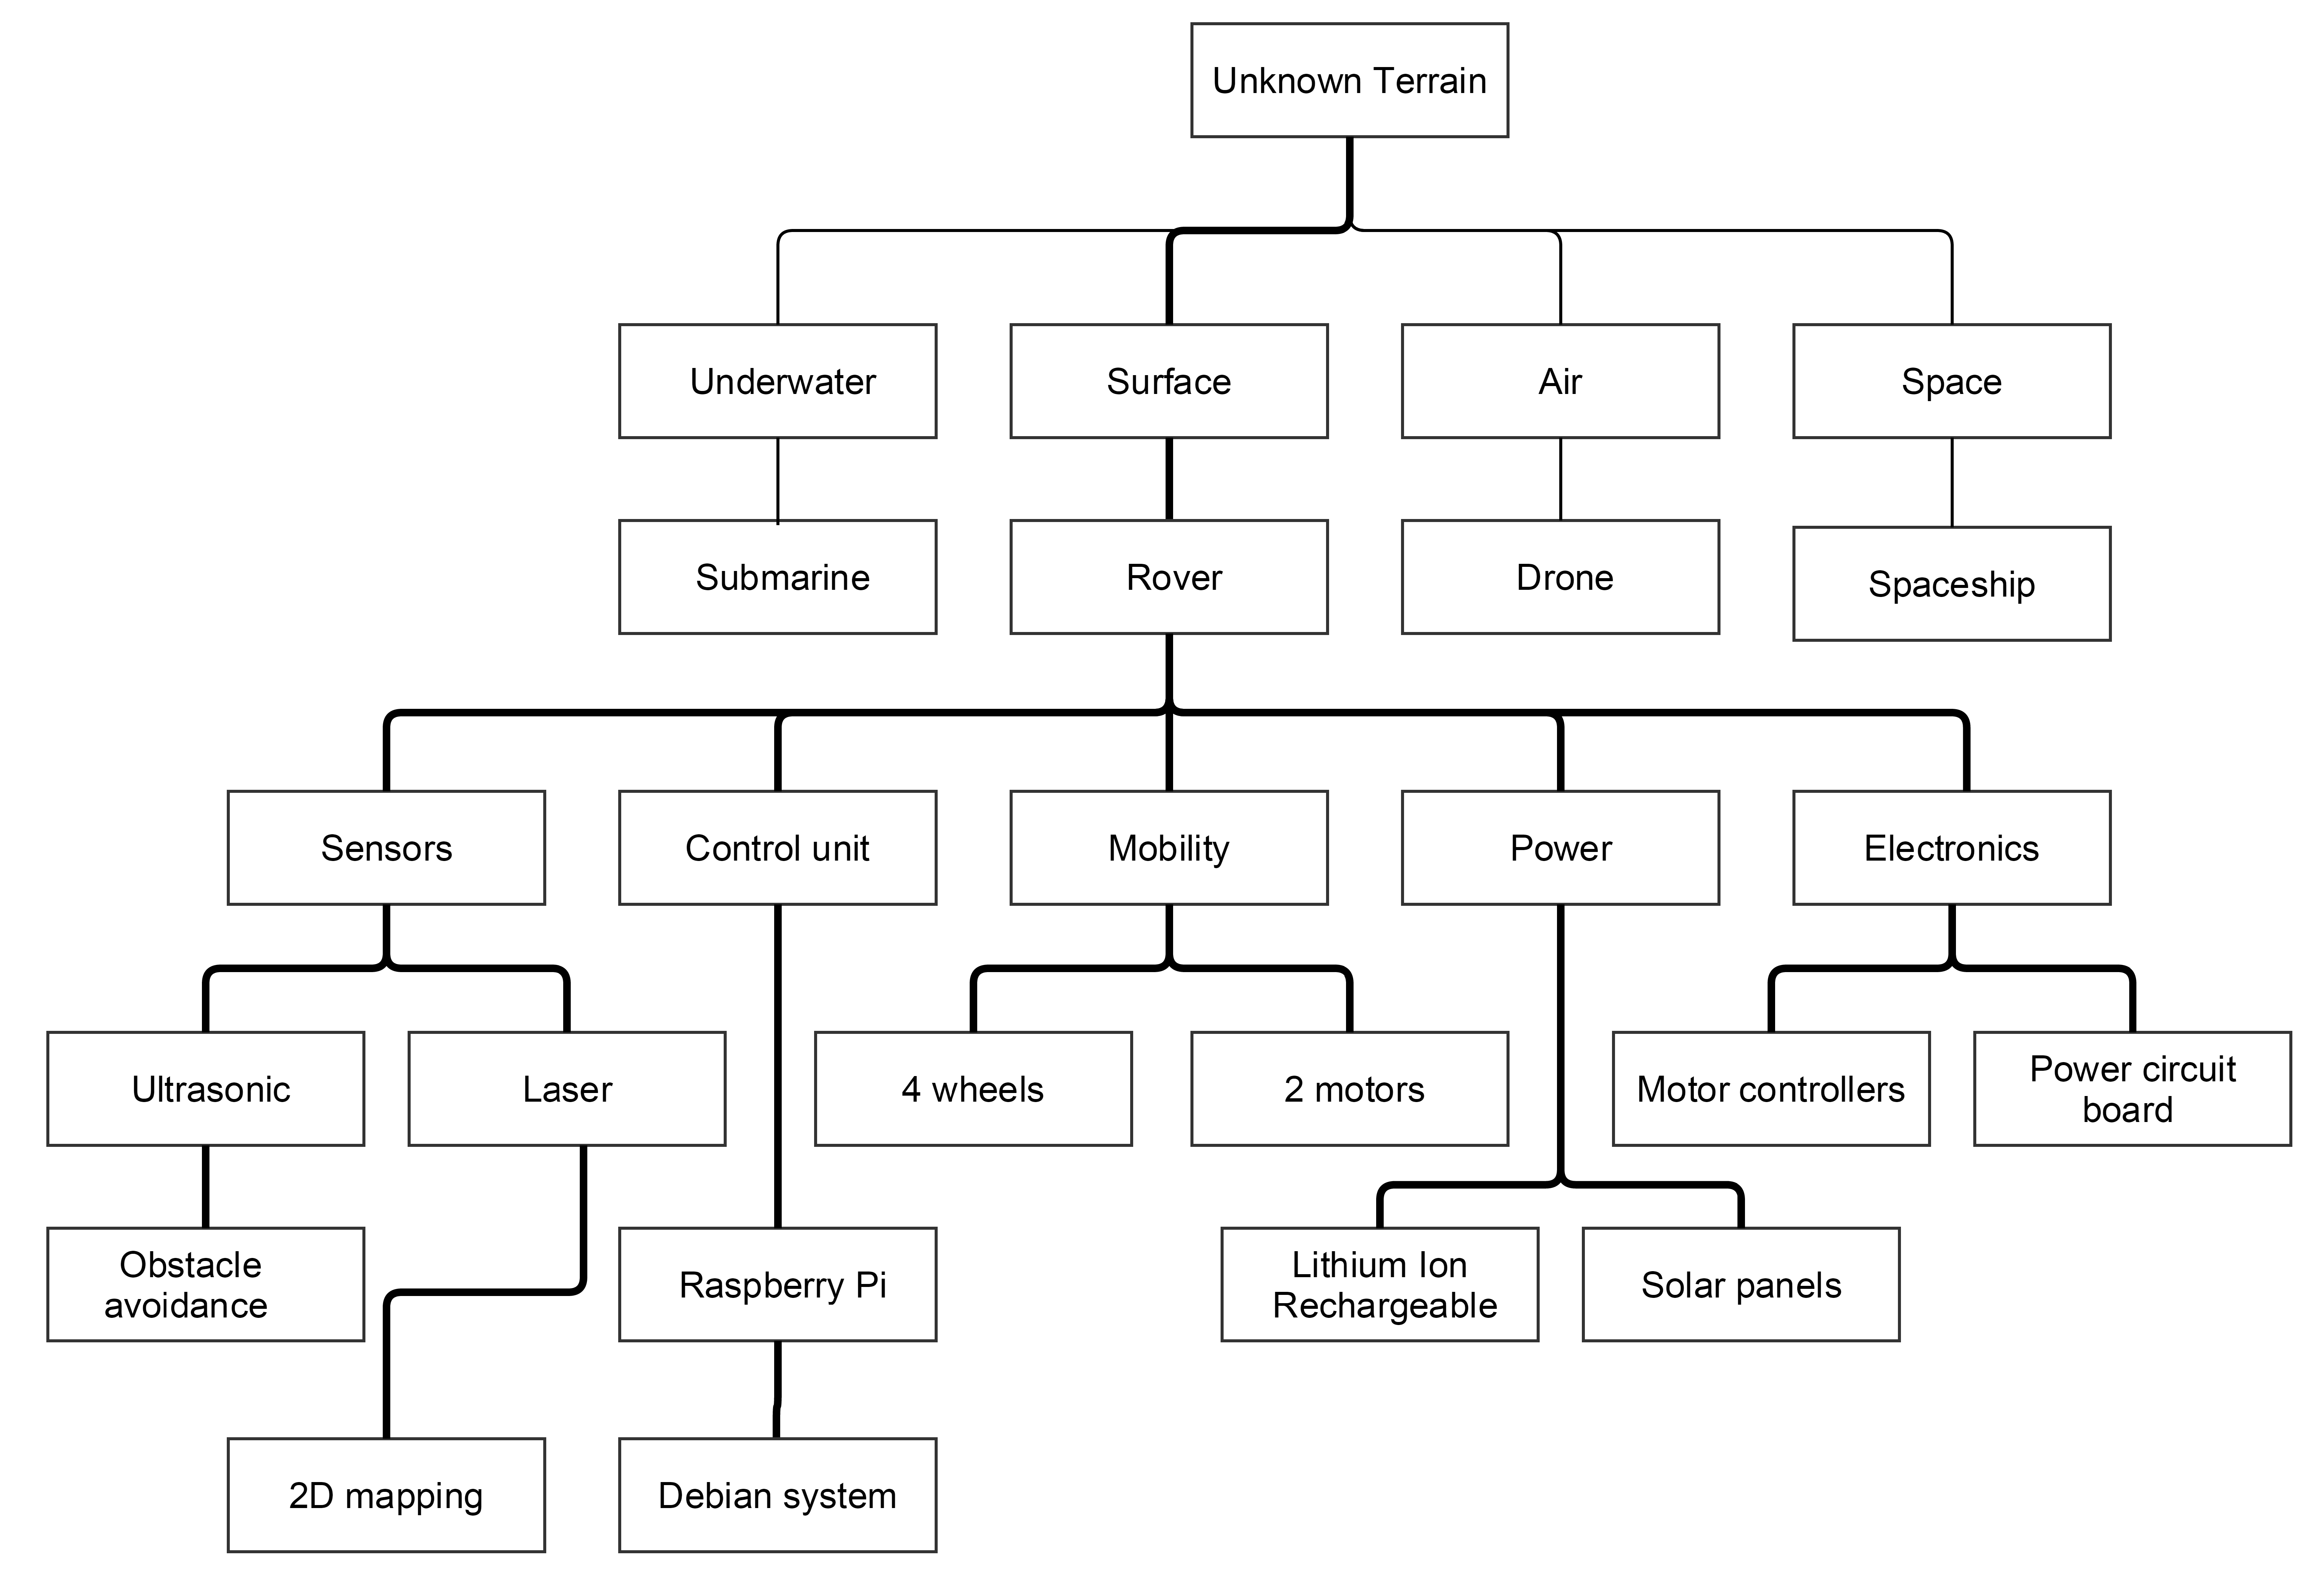
\includegraphics[scale=.1]{images/level3.png}
	\caption{Flowchart of the prototype idea.}
	\label{fig:level3}
\end{figure}

On this flowchart you can see how we expend from the level 1 flowchart in chapter 1.

\clearpage


%\section{Problem Delimitation}
Based on previous discussions, the following equipment has been selected:

\begin{description}
  \item[Rover:] \hfill \\
  A 4 wheel rover to move the sensor around.
  \item[Laser:] \hfill \\
  LIDAR-Lite rangefinder laser, used for distance measurement from points.
  \item[Brushless DC motor:] \hfill \\
  Used to spin the laser a full circle.
  \item[Ultra-sonic sensor:] \hfill \\
  For close proximity navigation.
  \item[Raspberry Pi:] \hfill \\
  As a control computer for navigation and processing of 2D map.
  \item[Optical-flow sensor:] \hfill \\
  Used for looking at a movement of the rover for reference points.
  \item[Motor controller:] \hfill \\
  Used to power the motors used on the rover.
  \item[Power source:] \hfill \\
  %TODO: Add missing information here%
\end{description}

\subsection{Prototype delimitation}
The main limiting-factor for us is time. In the time-frame of this project, we cannot build a full-scope product. Finding all the parts, ordering, and assembling them completely would take too long to complete and over our given budget. Furthermore, we do not have the tools or place to build a full-scope product, either. Hence we will build a prototype as a proof of concept using the means we have available.

For the prototype, we decided to use a laser to gather the data needed for a 2D map as a proof of concept, but at the same time allowing the capability of implementing cameras for 3D mapping. A laser can also be used for 3D mapping, but it would be easier to make a 3D map from cameras and using cameras would also give a better picture of the surroundings.

The optical flow sensor is used to determine reference points. We will be using Simultaneous Localization and Mapping (SLAM) technique for the mapping. The laser will be mounted on top and spin 360$^{\circ}$ using a brushless DC motor. The optical flow sensor will tell the system about the movement of the rover on a $XY$ grid, to determine the direction and distance the vehicle has travelled. 

This prototype will not have all the features we wish to have for the final product, but the goal is to show the interaction between an laser sensor for 2D mapping and a rover navigating through unknown terrain, using a Raspberry Pi.





\section{Hypothesis}

Due to the fact that our report deals with such a broad scope, we can not completely cover our initiating problem in such a short time. Therefore a hypothesis is used to measure the success of our project.
The solution to the initiating problem implemented in this project, will make an rover capable of 2D mapping an unknown terrain and be able to find its own path and navigate. Then return a usable 2D map of its surroundings from point A to B. The rover should also be capable of implementing equipment for 3D mapping.

\section{Problem Definition}

Problem Definition

%Chapter 4  ------------
\clearpage
\chapter{Development}\label{ch:development}

\section{Description}

Description and following chapters 

%\section{Design}

\begin{figure}[H]
    \centering
    \includegraphics[width=0.9\textwidth]{./images/fullscope1.PNG}
    \caption{Full-scope picture of the design }
    \label{fig:rfid1}
\end{figure}

The full-scope picture shows all connections in our design. The black dotted line is ground, yellow is 12V DC and red is 5V DC. Orange is used for data transfer. The 5V from the Arduino and D2 control the relay that opens for the 12V to the solenoid. There is a sensor in the lock that tells us when it is closed. That sends a signal to the Arduino in port D3. Ports A5 and A4 are connected to the LCD screen and it uses the $I^2 C$ protocol. Ports D9-D13 connects to the RFID reader using the UART protocol (Universal asynchronous receiver/transmitter).

\begin{figure}[H]
    \centering
    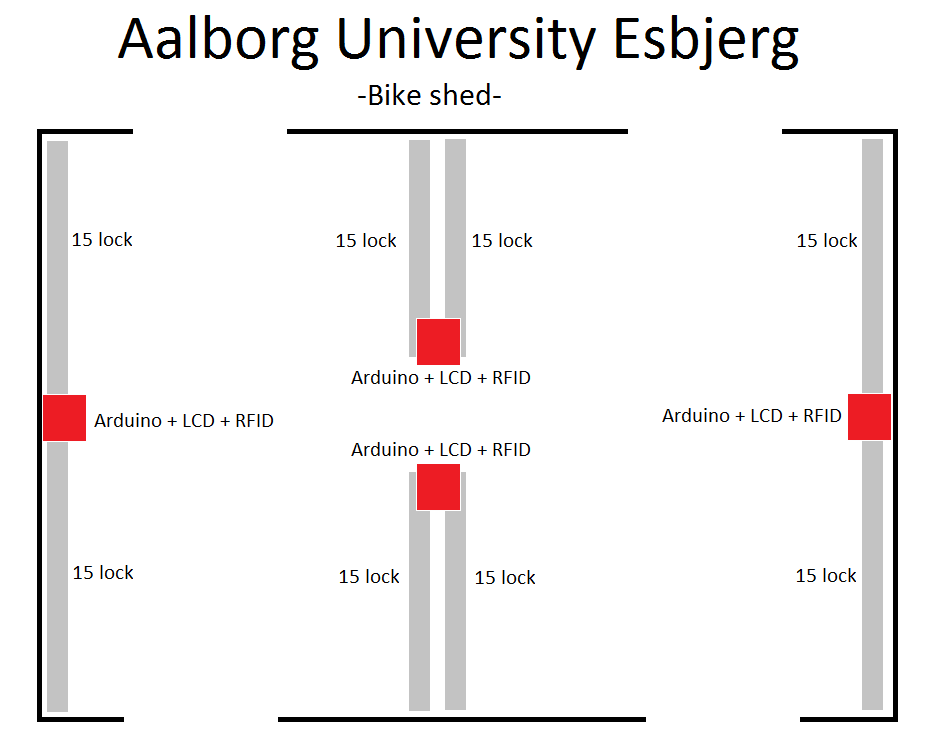
\includegraphics[width=0.5\textwidth]{./images/bikeshed.PNG}
    \caption{Aalborg University bike shed }
    \label{fig:bikeshed}
\end{figure}

Here is a basic concept idea of how we would implement the final design here in Aalborg University Esbjerg. For the final design a larger micro-controller would be necessary, like an Arduino MEGA, each MEGA could control up to 30 locks. All of the locks are controlled by a single RFID reader and one LCD screen. We would have our system on every other bicycle rack. So people could choose whether or not they wanted to use our system or their own locks. 

\subsection{Code}

\begin{figure}[H]
    \centering
    \includegraphics[width=1.1\textwidth]{./images/codeflow.PNG}
    \caption{Flowchart of the code used }
    \label{fig:codeflow}
\end{figure}

The flowchart shows a general idea of how our code will work. It will have two main functions. One is for locking new bicycles to the rack and the other is to unlock the bicycle. On the left side of the flowchart you can see a timer set t=30. If 30 seconds pass and no new RFID card is scanned to be associated with a lock, then the lock will automatically unlock. If a RFID card is read it will ignore to auto-unlock and continue with the program. 

\begin{algorithm}[H]
\caption{RFID bike lock}
\begin{algorithmic} 
\STATE LCD display - Welcome screen
\STATE
\WHILE{touch sensor pressed $= 1$}
\STATE sensor \textbf{X} = lock \textbf{X} 
\STATE LCD display - Is your lock number \textbf{X}? Then please read RFID card.
\STATE
\IF{RFID tag is valid}
\STATE lock \textbf{X} connects to RFID tag
\STATE timer $= 0$
\STATE LCD display - Bike lock \textbf{X} is now locked. Thank you
\STATE touch sensor pressed $= 0$
\ELSIF{RFID tag is invalid}
\STATE unlock bike lock \textbf{X}
\STATE LCD display - ERROR invalid or used card, Try again.
\ENDIF
\STATE
\IF{timer $= 30000$}
\STATE unlock bike lock \textbf{X}
\STATE LCD display - Bike lock \textbf{X} was not locked. Try again.
\ELSE
\STATE timer $=$ timer $+1$
\ENDIF
\STATE
\STATE delay $1$
\ENDWHILE
\STATE
\IF{RFID read}
\IF{RFID tag used}
\STATE unlock bike lock \textbf{X} that is connected to that card
\STATE LCD Display - Bike lock number \textbf{X} is now unlocked. Thank you.
\ELSE
\STATE LCD display - ERROR invalid or used card, Try again.
\ENDIF
\ENDIF
\end{algorithmic}
\end{algorithm}

\clearpage

\subsection{Locking enclosure}

The main characteristics of the prototype lock design are:

\begin{enumerate}	
	\item Solenoid based
	\item Switch as a locking sensor
	\item Easy to build wooden case
	\item Additional space to fit relay and cables
	\item Covered by Plexiglas
\end{enumerate}

\begin{figure}[H]
	\centering
	\includegraphics[width=0.6\textwidth]{images/design/lockwood.png}
	\caption{CAD drawing of the lock design}
	\label{fig.cadlock}
\end{figure}

During the design phase we assumed that this lock would be mounted directly on a bicycle rack. The red plug connects to a chain, which is secured to the rack, allowing a bicycle to be locked to it. When the lock is unlocked, the red plug will fall out of the enclosure from gravitational force. This design feature allow the plug to be kept in place while the user is scanning their card. The end of the plug is rounded to make it easier to insert the plug into the locking enclosure.


%\clearpage
\section{Specifications}

Components:
\begin{description}
      \item[RFID Reader:] \hfill \\
        An RFID reader that can read RFID-tagged cards. 5.3 dollars. \cite{specrfid}
      \item[Solenoid:] \hfill \\
        A solenoid, similar to a door strike. It takes 9-12V. 15 dollars. \cite{specsolenoid}
      \item[Micro-controler:] \hfill \\
        Arduino UNO. Takes 5V-20V. 17 pounds. \cite{specarduino}
      \item[Relay:] \hfill \\
        Used to control the solenoid. \cite{specrealy}
      \item[Switch:] \hfill \\
        A small contact that closes whenever the lock-head is inside the case. \cite{specswitch}
      \item[LCD Screen:] \hfill \\
        A 16x2 LCD screen that relays information to the user. 24.4 pounds. \cite{speclcd}
      \item[Chain:] \hfill \\
        A 1.5m steel chain. Each link is 1.5cm wide, and 3mm thick.
      \item[Lock Head:] \hfill \\
        A simple lock head made out of plywood. It locks into the wooden casing. Built by us.
        2x2x16cm
      \item[Wooden Casing:] \hfill \\
        A simple casing made out of plywood. Holds the solenoid and relay. Built by us.
        10x18x4cm
      \item[Electronics box:] \hfill \\
        A box that holds the micro-controller, LCD, and RFID reader. 17x12x5.5cm

\end{description}
Overall, the electronics box and wooden casing are mounted on a metre high, half-metre wide plywood panel, which is attached to a metre long bike rack.
\clearpage


%\section{Documentation}

The development of our product started out with early-prototyping of the code and the individual components. Right after the research and initial analysis was completed, we started looking into running the individual components and searching for libraries that we needed to use. This helped us to identify problems like lack of documentation of LCD libraries for the Arduino MEGA board, which we considered to use at some point of our research. 


These smaller component-prototypes eventually became part of our prototype code.


The code for the prototype only works for the desired single-lock prototype. It can take any student card and associate it with a lock. But it will only store the card information when the lock is locked and delete the information when its unlocked. For future work we would use a centralized database to deal with multiple locks and cards.

\subsection{Code}

%---------------
	
\lstinputlisting[firstline=176, lastline=221, title=Prototype main loop]{./code/RFID_Prototype.cpp}

The main loop in the prototype code always checks if there is a new RFID tag read, or if a lock recently has been locked. If nothing is happening it will show the welcome screen. The main loop then has two main if statements. The first if statement checks if there is a RFID card read by the system and the second if statement checks if the sensor in the enclosure has been activated from the locking-peg.

 
If an RFID tag is read, it will check if it is a valid and connect it to a lock. If the card already is connected to a lock, the display will show a message to the user that the lock is unlocked and then unlocks the bicycle. 


If the sensor in the enclosure registers a new lock it will ask the user to scan their RFID tag/card. It will check if the card is valid or connected to another lock. It will do this for 30 seconds. If no valid RFID card is read in 30 seconds it will unlock the lock and display it to the user. The system has this feature in place to avoid people locking all the locks without associating them with a RFID card of some sort.


If a valid one is read it will display a message to the user that the system is locked and that their card is associated with that specific lock.


The main loop also addresses input errors. One is if at any time an RFID card is read that is invalid for this system and another is if the user is trying to lock the second bike lock with the same RFID card it will display an error message to the user.

\clearpage

%---------------

\lstinputlisting[firstline=223, lastline=233, title=Prototype sensorRead function]{./code/RFID_Prototype.cpp}

The function $sensorRead()$ checks if the lock has been locked. The end of the lock has a sensor and it will notify the program what lock has been locked. The program then goes to check for a new RFID tag for 30 seconds. If no RFID tag is scanned it will open the lock again. If a new RFID tag is entered it will change the number in the array $lockCheck[]$ from 0 to 1. So the program will ignore a previously locked lock.


%---------------


\lstinputlisting[firstline=414, lastline=428, title=Prototype lockLock function]{./code/RFID_Prototype.cpp}

Te function $lockLock()$ displays a message to the user that the lock is now locked and changes the array $lockCheck[0]=0$ to $lockCheck[0]=1$. That is done to prevent the system to check multiple times on the same lock that has been connected to an RFID tag.


%---------------

\lstinputlisting[firstline=280, lastline=298, title=Prototype getID function]{./code/RFID_V1.cpp}

The function $getID()$ checks if a new RFID tag is read by the RFID reader. If so it checks if the card is of the right type. It then writes it to the array $readCard[]$. It only stores 4 bytes of information, which is the ID of the card. The program ignores all of the other user data. In future versions we can hash the information, hashing is encrypting the data so that even if someone gets the data it is unusable.
  

%---------------

\lstinputlisting[firstline=435, lastline=449, title=Prototype checkTwo function]{./code/RFID_V1.cpp}

The function $checkTwo()$ compares two arrays together to see if they have the same data. The function compares the $storedCard[]$ array to $readCard[]$, to see if the card that is read is in the system or not. For future systems where there is more than one lock, it is also necessary to compare the pointer array $lock[]$ to $readCard[]$ and then open the connected lock to that RFID tag.

\clearpage

%---------------

\lstinputlisting[firstline=523, lastline=530, title=Prototype isMaster function]{./code/RFID_V1.cpp}

The function $isMaster$ only checks if the RFID tag that was read is the master card and uses the $checkTwo[]$ function to do that. Master card is used by the main user to help with the system if an error comes up or a card is lost.


%---------------

\subsection{Build}

The prototype case for the locking device is primarily built using plywood, a 12V solenoid, a mechanical relay, a switch and a Plexiglas cover.
 
\begin{figure}[H]
	\centering
	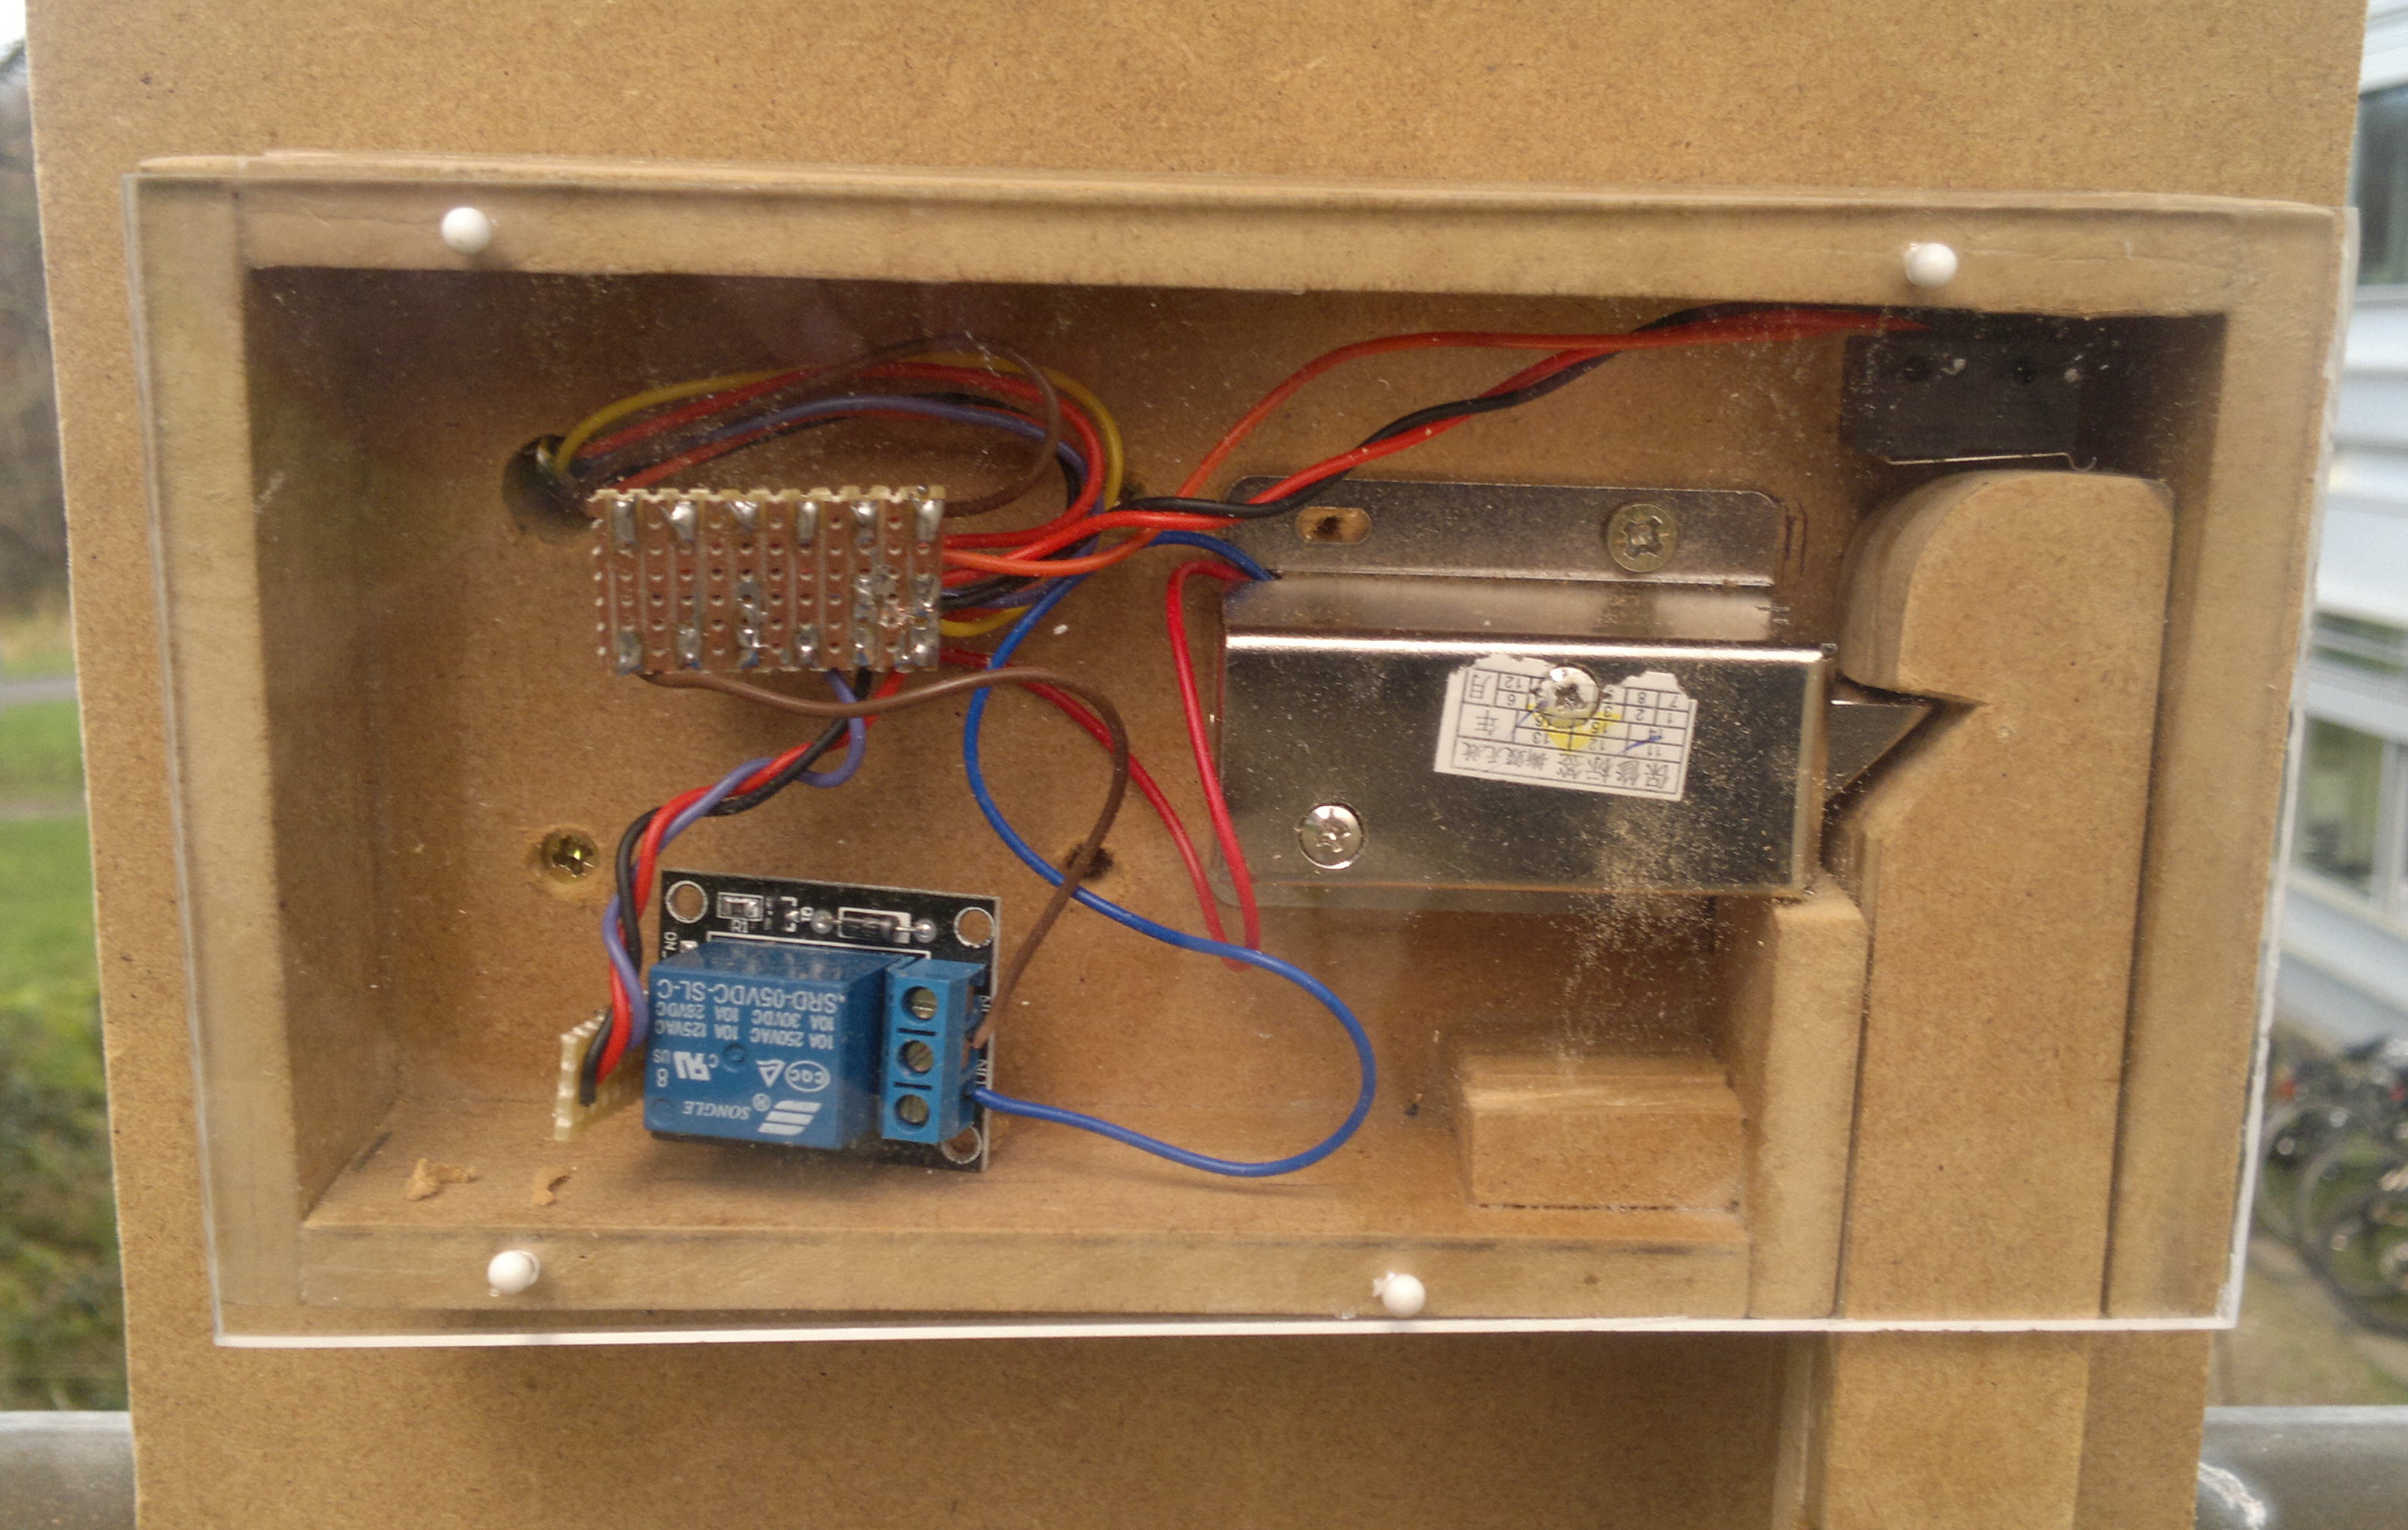
\includegraphics[width=0.6\textwidth]{images/desc/lock.jpg}
	\caption{Picture of lock}
	\label{fig.lock}
\end{figure}


The main prototype box contain an Arduino Uno development board (containing Atmel micro-comtroller), a RFID reader and a LCD 16x2 screen. They are placed in a ABS electrical box in which we have cut hole fitting the display. A RFID reader is located on the other side of the box, inside, under the label.

Both the locking enclosure and the case containing the micro-controller and electronic components are secured to a plywood wall and is mounted to the bicycle rack. The box containing the electronics is mounted on an extension that is tilted at an $45\,^{\circ}$ angle, making the display text more readable. The case containing the locking mechanism is mounted directly on the wall.

\begin{figure}[H]
	\centering
	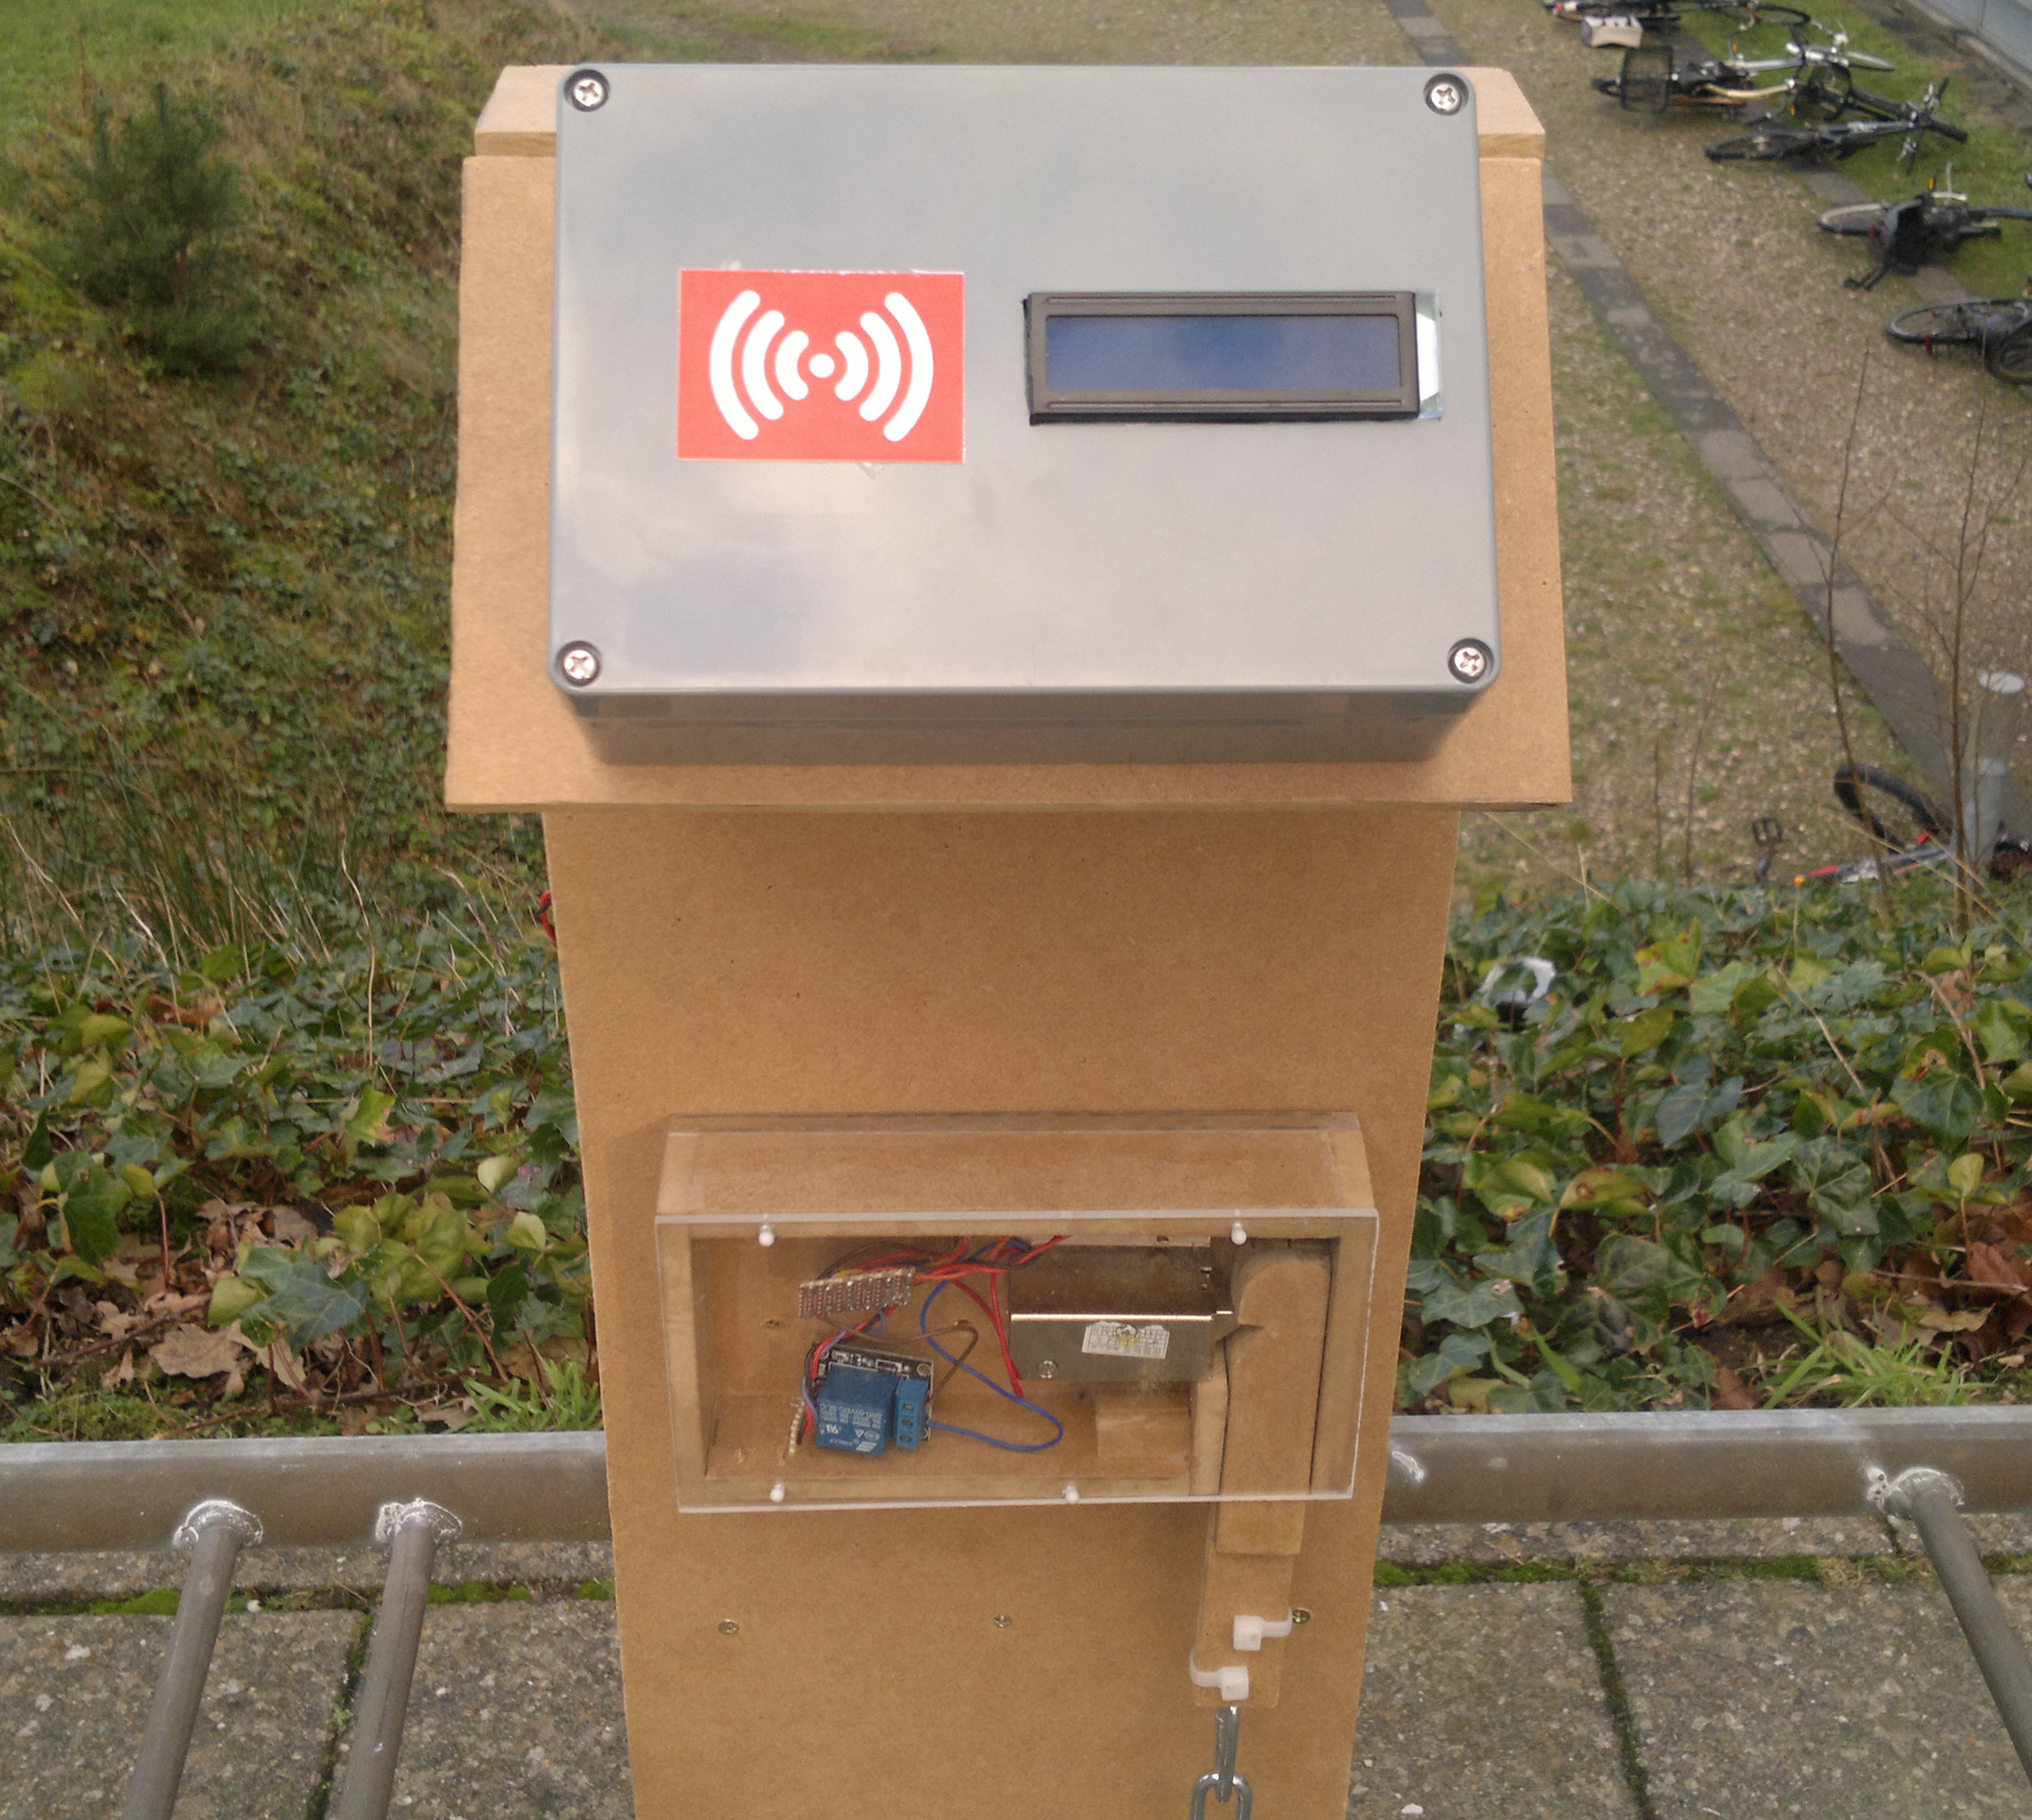
\includegraphics[width=0.6\textwidth]{images/desc/boxes.jpg}
	\caption{Picture of components}
	\label{fig.rack}
\end{figure}


\begin{figure}[H]
	\centering
	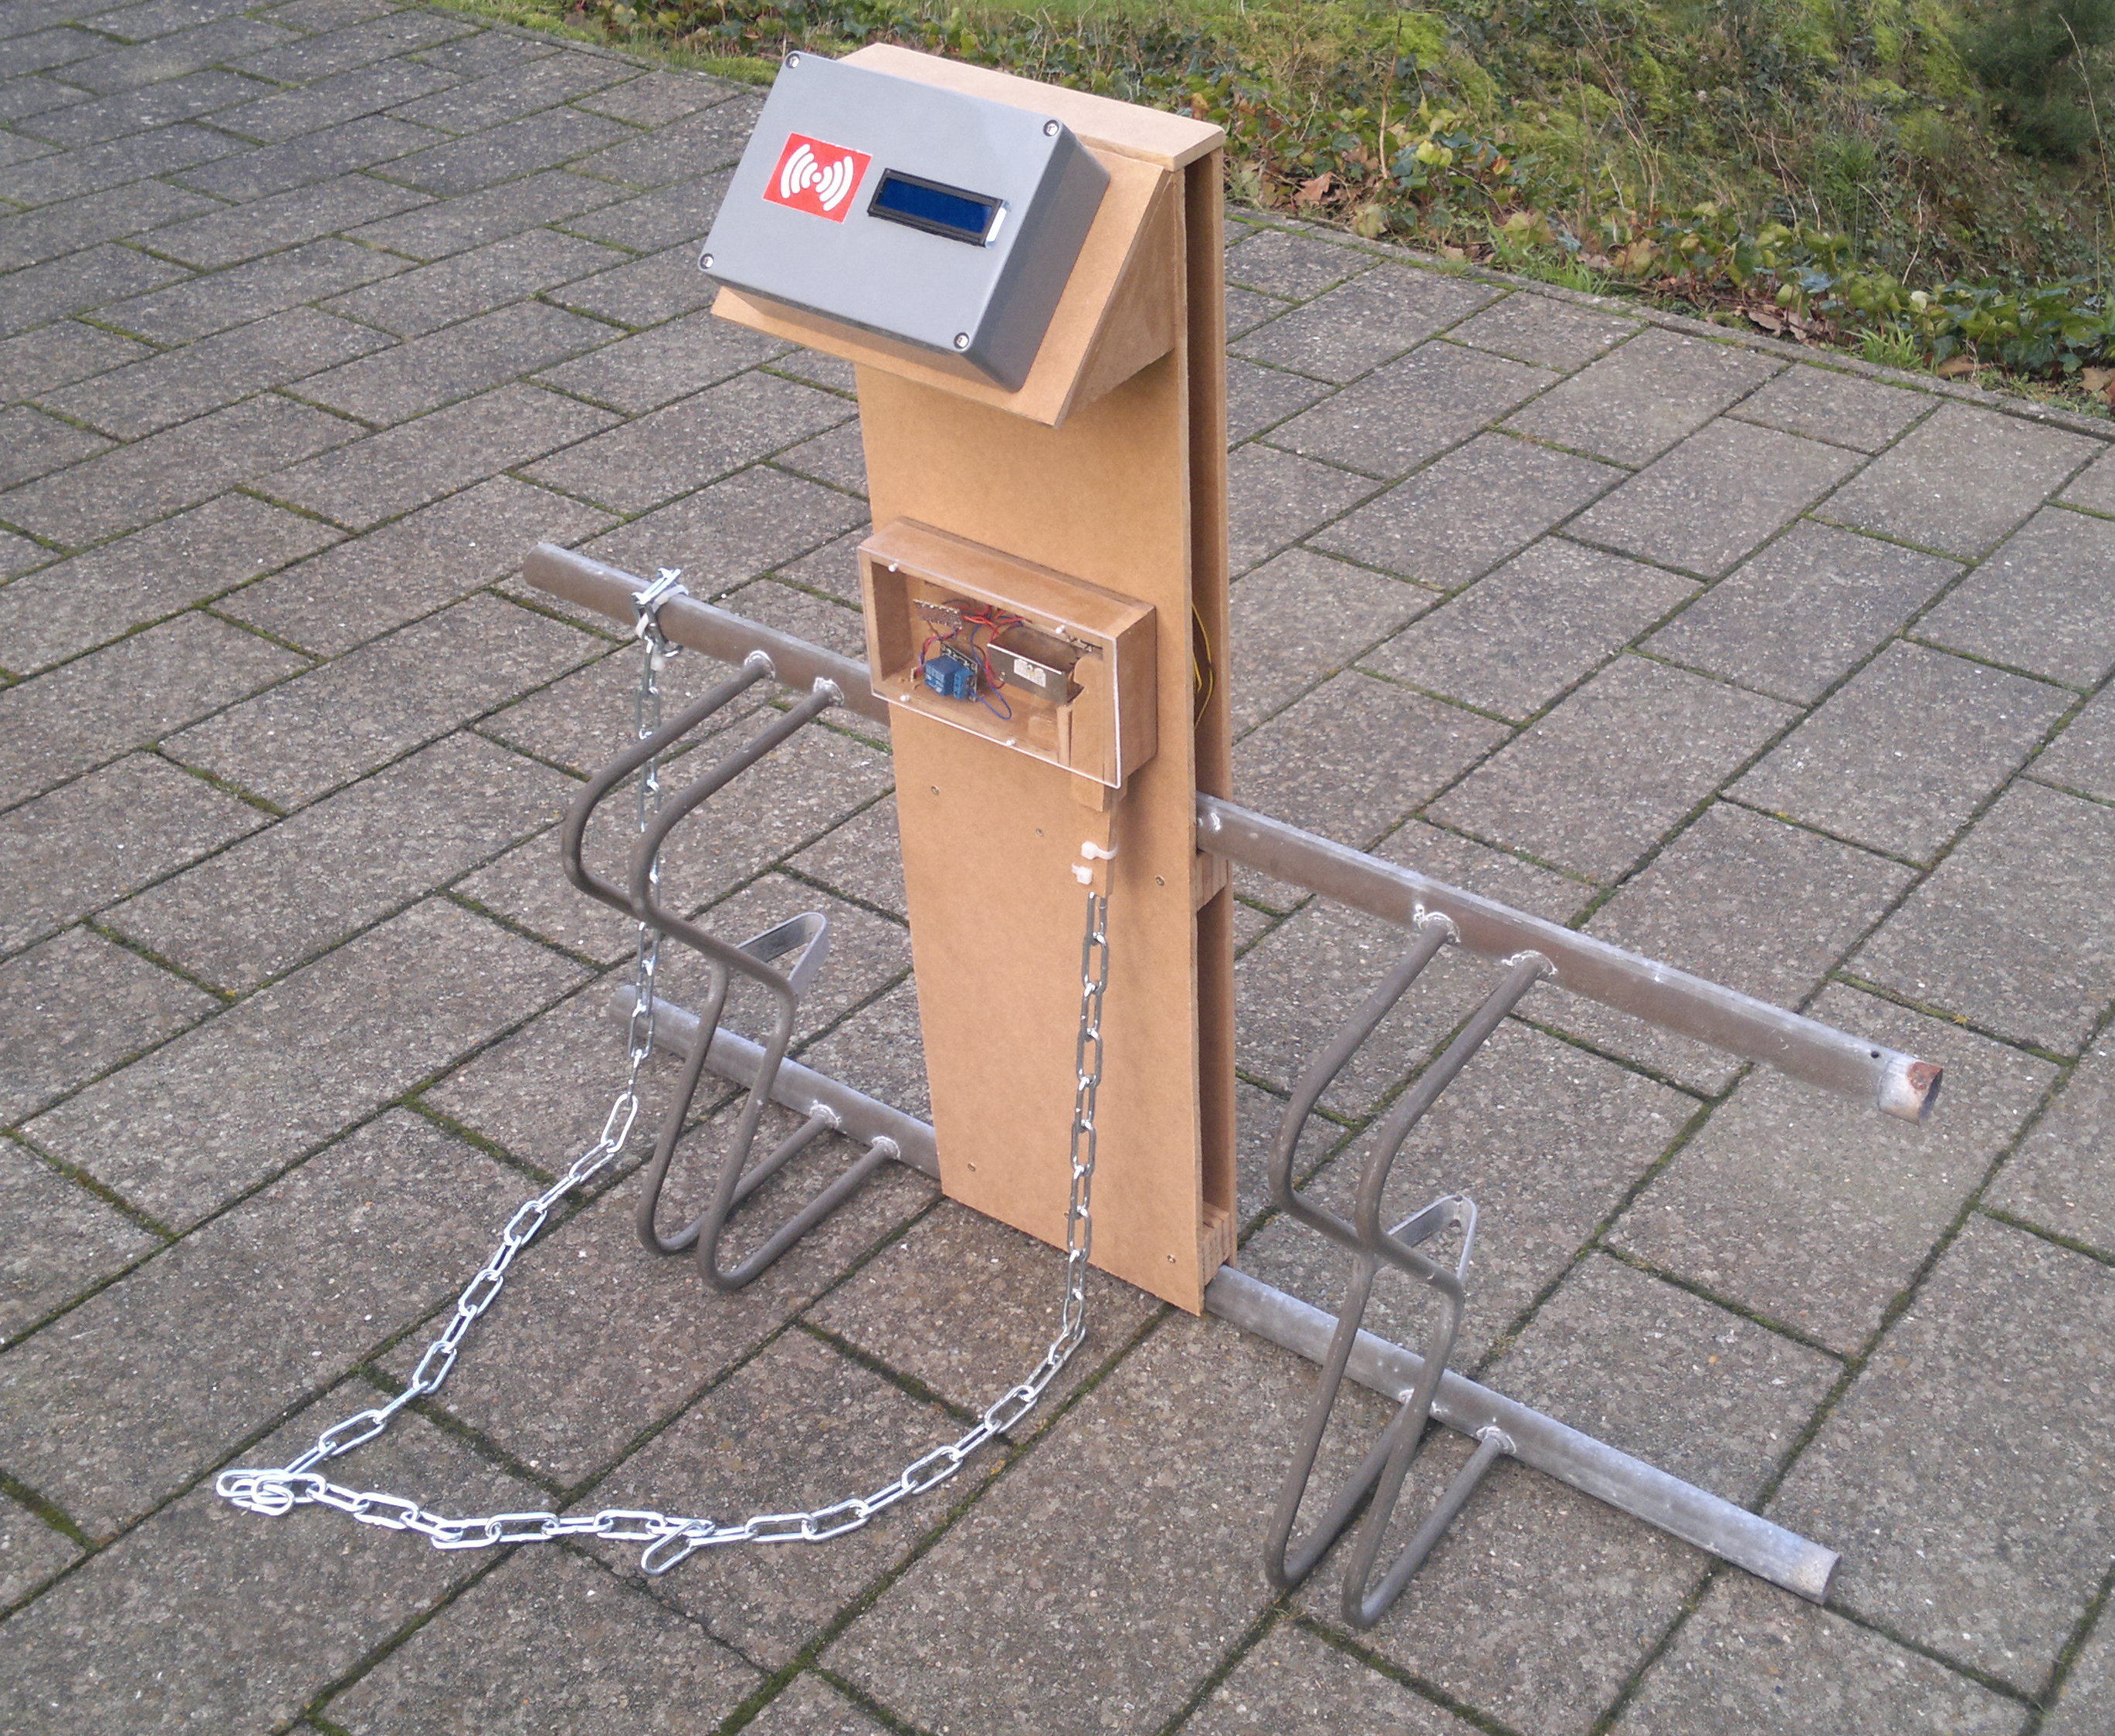
\includegraphics[width=0.6\textwidth]{images/desc/full.jpg}
	\caption{Picture of prototype rack}
	\label{fig.rack}
\end{figure}

The components in the main box are connected by plug-in cables and soldered where needed, according to our design. The lock case and the wall is made of plywood using basic tools. The lock case construction is glued and nailed together, built after a slightly altered design, due to the fact that more advanced tools were not available. 


%\clearpage
\section{Testing}

To ensure that our prototype fulfills every requirements we set up in Chapter 3, we set up some testing scenarios, which we used to test the functionalities of our prototype. This scenario is made out of a maze/location like this

[top-view of maze/room here]

%TODO: Create top-view of room and conclude of test

%TODO: Show test findings

Therefore we can conclude that the test requirements set previously are all passed.

\begin{table}[H]
	\begin{tabular}{|l|l|}
		\hline
		\textbf{Requirement} & \textbf{Test} \\ \hline
		The rover can be controlled using a remote device. & PASSED/FAILED \\ \hline
		The rover should navigate autonomously through a maze. & PASSED/FAILED \\ \hline
		The laser sensor should make a usable 2D map of its surroundings. & PASSED/FAILED \\ \hline
	\end{tabular}
\end{table}



%Chapter 5  -----------
\clearpage
\chapter{Discussion}\label{ch:discussion}

Discussion 

%Chapter 6  -----------
\clearpage
\chapter{Conclusion}\label{ch:conclusion}

Conclusion 

%Latex part of the report -------------

%\chapter{\LaTeX}\label{ch:latex}

%%Information from the LaTeX lecture 3 regarding the needed LaTeX section:
%
%1. Add chapter named LATEX after conclusions (one page)
%2. Write briefly about why you chose to use LATEX
%2.1 Bullet list on things/ideas to improve in this course to make
%transition from Word easier
%2.2 Enumerated list on which areas you still feel uncomfortable
%2.3 From your experience, write bullet list on LATEX strong points
%2.4 From your experience, write bullet list on LATEX weak points

%\chapter(LaTeX)

One of the main reasons we chose to use \LaTeX\ was because of version control. Using Word or something similar sets some unavoidable limitations when it comes to doing research and writing a report. 
Another great benefit with using \LaTeX\ in our group is the OS Independence, in our group of 5 members there is 3 different operating systems.

Improvement suggestions:
\begin{itemize}
	\item More exercises
	\item More challenges
	\item Clarity on the steep learning curve and why it's worth transitioning
\end{itemize}

Areas of which we still feel uncomfortable:
\begin{enumerate}
	\item Creating templates
	\item Manipulating with the AAU template
\end{enumerate}

The strong points of \LaTeX:
\begin{itemize}
	\item The ability to use version control (git/SVN)
	\item Packages
	\item Customizability
	\item Open-source and OS-independent
\end{itemize}

The weak points of \LaTeX:
\begin{itemize}
	\item The syntax is too verbose
	\item Hard to debug errors
	\item Differences in IDE capabilities on different platforms.
\end{itemize}


%--------------------------

%Chapter 7  -----------
\clearpage
\chapter{Perspective}\label{ch:perspective}

perspective 

\clearpage
\Urlmuskip=0mu plus 1mu\relax
\sloppy
\bibliographystyle{unsrt}
\bibliography{citations}{}

%Other chapters ------------
\chapter{Appendix}\label{ch:appendix}
\section{Personal learning goals}\label{appendix:personal-learning-goals}

\subsection{Antal János Monori}
\subsubsection{P2 learning goals}
\begin{itemize}
	\item Gain general knowledge of 2D/3D mapping using reference points
	\item Learn to apply analog sensors, more in terms of navigation on a rover
	\item Learn to use sensors in Python on a Raspberry Pi by the end of the P2 project
\end{itemize}
\subsubsection{Semester learning goals}
\begin{itemize}
	\item Learn to do 2D/3D modelling using CAD software by completing the 3D CAD class
	\item Learn and understand the basics of electrical circuits during the development phase of our P2 project
	\item Get familiar with VHDL and ABEL syntax-wise by the end of May.
\end{itemize}

\subsection{Emil Már Einarrson}
\subsubsection{P2 learning goals}
\begin{itemize}
	\item Learn mapping in 2D using a laser sensor [End of P2 semester]
	\item Learn more about robot control using a raspberry pie [End of P2 semester]
	\item Learn how sensors work differently in space and other planets. Ultrasonic and lasers [End of March]
	\item Learn about different sensors and measurements you can use to get a reference points for mapping [End of April]
\end{itemize}
\subsubsection{Semester learning goals}
\begin{itemize}
	\item Learn more about analog and digital circuits [End of P2 semester]
	\item Learn more CAD drawing [End of P2 semester]
\end{itemize}

\subsection{Gustavo S. Buschle}
\subsubsection{P2 learning goals}
\begin{itemize}
	\item Learn how to construct a 2D or 3D map based on point-data gathered from rangefinders, by the need of the development.
	\item Learn how effectively use a map for autonomous navigation, by the end of the development.
\end{itemize}
\subsubsection{Semester learning goals}
\begin{itemize}
	\item Learn how to schedule tasks in a distributed fashion.
	\item Learn how CPU instructions are translated to circuit operations.
\end{itemize}

\subsection{Thomas Thuesen Enevoldsen}
\subsubsection{P2 learning goals}
\begin{itemize}
	\item Gain knowledge about how sensors work differently in space and other planets [During our initial research]
	\item Apply different kinds of sensors [During the development chapter]
	\item Gain comprehension of 2D/3D mapping [During the entire project]
	\item Gain knowledge about Electrical circuits [During the entire project]
	\item Gain knowledge about Analog and Digital circuits [During the entire project]
	\item Become better at programming [During the development phase]
	\item Become better at collaboration and group management [During the entire project]
\end{itemize}
\subsubsection{Semester learning goals}
\begin{itemize}
	\item Apply 3d modelling using cad software [During the free-study activity and P2 project]
\end{itemize}

\clearpage

\section{Curriculum learning goals}\label{appendix:curriculum-learning-goals}
\subsection{Knowledge}
\begin{itemize}
	\item Shall have gained experience with theories and methods of calculation and simulation of linear electronic circuits, linear electro-mechanical systems, and/or other linear systems
	\item Shall have acquired knowledge of methods for analysis of linear dynamic systems, including electronic circuits, described by differential equations
	\item Shall have gained insight into basic feedback theory and its applications in electronic systems
	\item Must master calculations with complex numbers, as used within the field of electronics
	\item Shall have knowledge of recognized standards for documentation of electronic circuits, including electrical diagrams, PCB layout, etc.
	\item Shall be able to demonstrate knowledge of theory and method to the extent of being able to explain and justify the project's theory and methods, including both selection and de-selection.
	\item Shall master the relevant terminology
\end{itemize}

\subsection{Skills}
\begin{itemize}
	\item Shall have understanding of basic theories behind simple electronic components such as resistors, capacitors, operational amplifiers, etc., including calculation of these components
	\item Shall be able to identify, analyse and formulate issues within the discipline through the use of contextual and technical analysis methods
	\item Shall, based on the above, be able to create requirements and test specifications that enable the completed system to be tested rigorously
	\item Shall be able to use mathematical theories and methods to analyse problems involving linear dynamic components
	\item Shall be able to simulate and design simple analog circuits, allowing specific, desired properties to be achieved.
	\item Shall be able to design and implement basic analog and digital circuits and demonstrate that these work as intended
	\item Shall be able to document and disseminate knowledge and skills with proper use of terminology, orally and in writing through a project report
	\item Shall be able to analyse and reflect upon his/her own learning process using appropriate methods of analysis and experience from P0 and P1
	\item Shall be able to analyse a technical-scientific problem under consideration of technological and societal contexts, and assess the technological and social consequences of proposed solutions.
\end{itemize}

\subsection{Competences}
\begin{itemize}
	\item Must be able to demonstrate, independently and in groups, the ability to plan, organize, implement and reflect upon a project that is based on a problem of relevance to society or industry, in which analog electronic devices play a central role
	\item Must have acquired, independently and in groups, the ability to obtain the necessary knowledge of a contextual as well as of technical nature, and be able to formulate models of limited parts of reality to such a level of abstraction that the models can be used in the design, implementation and test of a comprehensive system to meet given requirements
	\item Must be able to evaluate and take responsibility for science and technical solutions in a societal perspective.
	\item Must be able to generalize and reflect upon the experience with project planning and cooperation for the further study acquired during the project work
\end{itemize}

\clearpage
\section{Kanbanflow}\label{appendix:kanbanflow}

\begin{figure}[H]
	\centering
	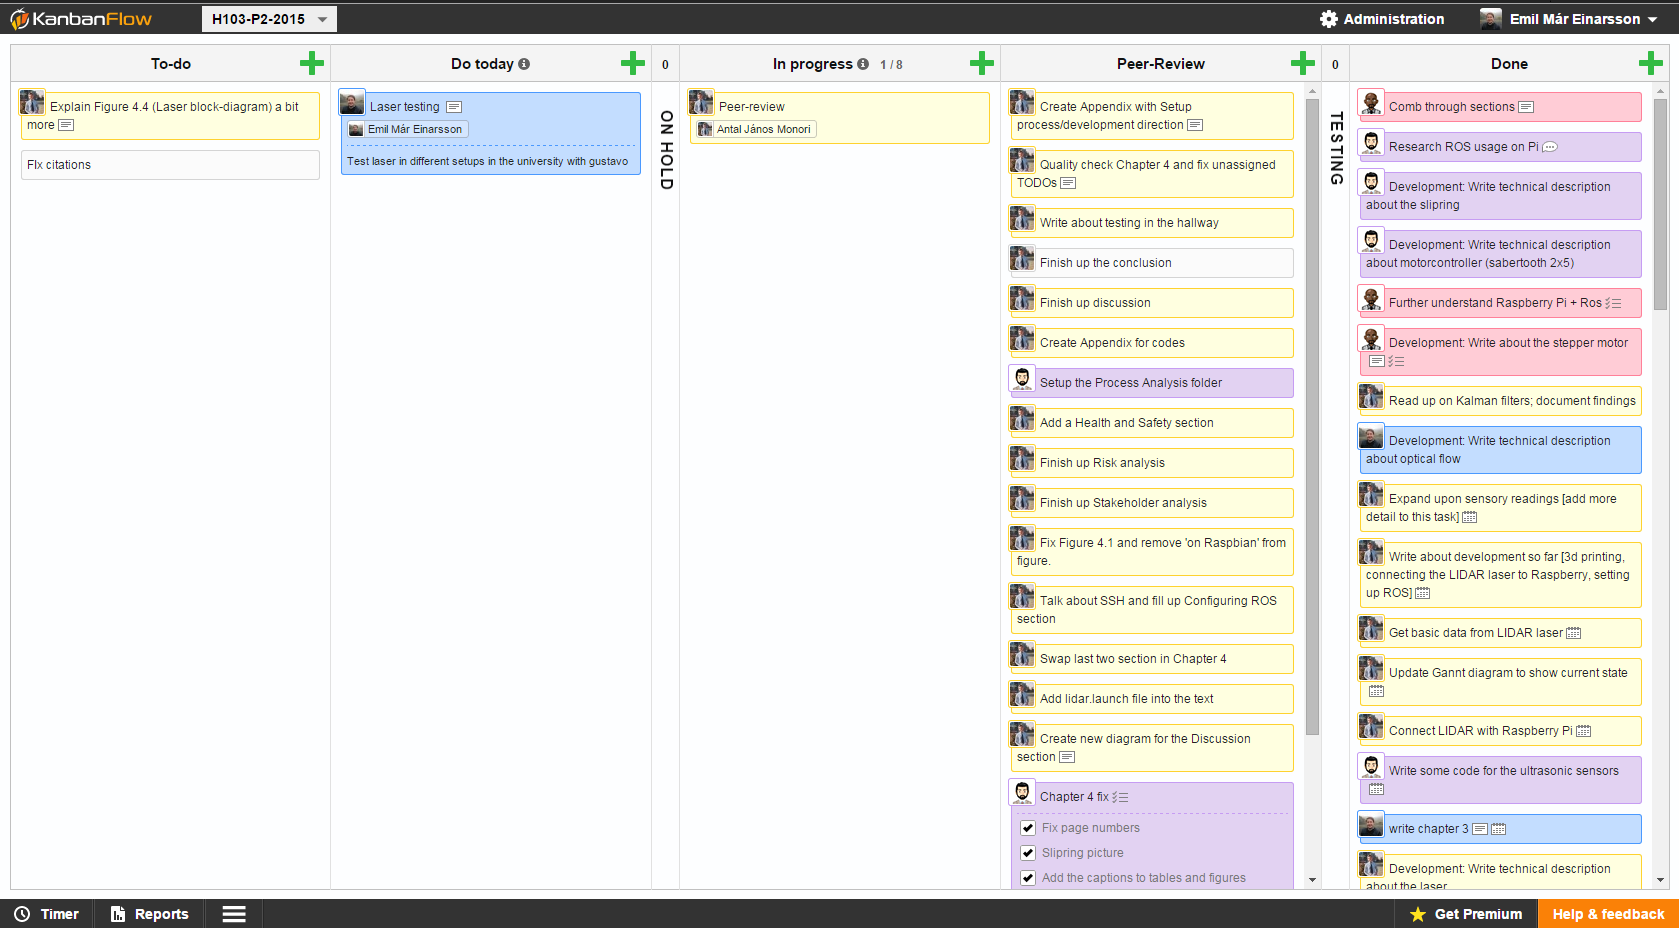
\includegraphics[width=1\linewidth]{images/kanban.png}
	\caption{Screenshot from online kanbanflow.}
	\label{fig:kanban}
\end{figure}

\clearpage
\section{Github}\label{appendix:github}

\begin{figure}[H]
	\centering
	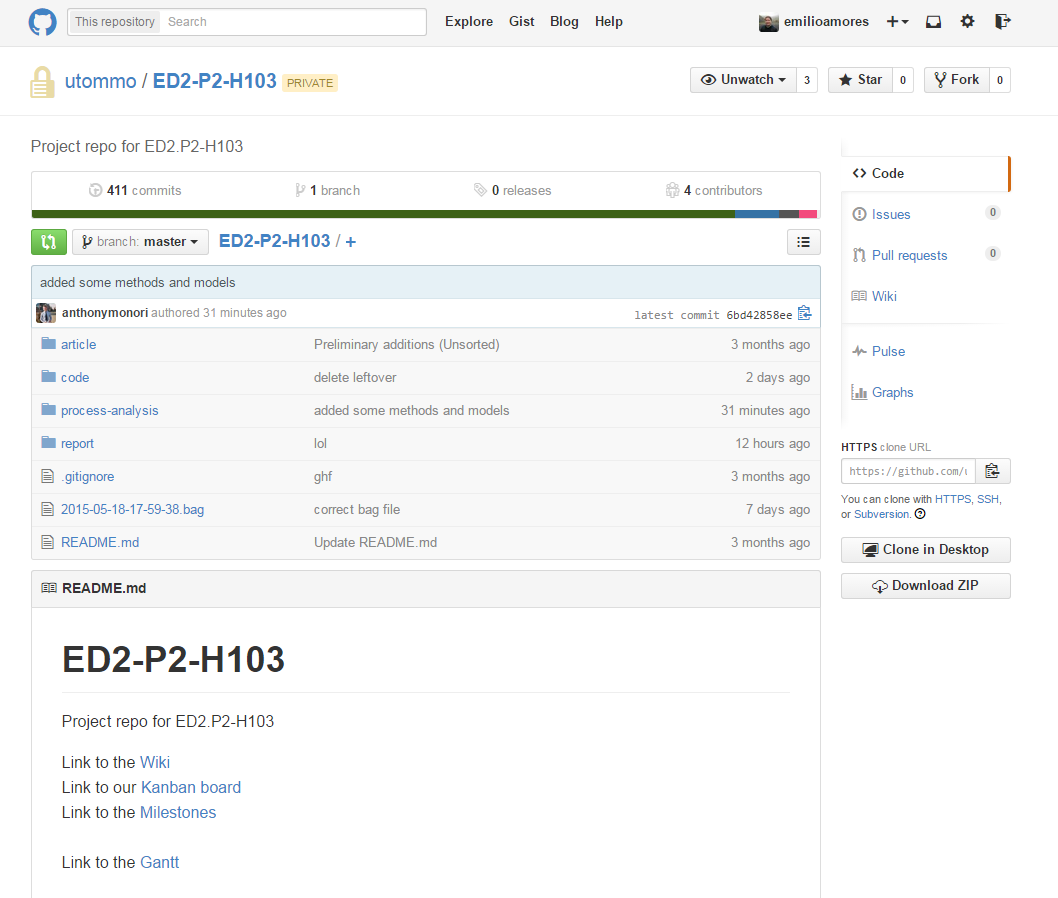
\includegraphics[width=1\linewidth]{images/github.png}
	\caption{Screenshot from the Github wiki.}
	\label{fig:github}
\end{figure}

\clearpage
\section{Group contract}\label{appendix:group-contract}

\begin{enumerate}
	\item Honesty is expected from everybody.
	\item Deadlines must be communicated up front, visualized and kept in mind during the whole project period.
	\item Postponing deadlines must be communicated at least halfway through the progress.
	\item During each meeting, deadlines must be set and followed up on.
	\item If the deadlines are not met, it will be brought up at the next strategy meeting.
	\item We aim to work at our full potential and get an acceptable grade, 7.
	\item All members take personal responsibility in achieving the learning goals, but it is expected.
	\item We keep all communications in English.
	\item We must notify each other when running late prior to the start of a meeting. Any notification after a meeting's start time is not taken into consideration.
	\item Wait time for late runners is 10 minutes maximum, with reasonable motive, otherwise we carry on without the missing participant(s).
	\item We penalize late runners or group members who do not comply with any of the following agreements:
	\begin{itemize}
		\item First strike: Warning + Reimbursement in form of beverages for all group members
		\item Second strike: Serious conversation within the team
		\item Third strike: Bringing the issue to our supervisor's attention
	\end{itemize}
	
	\item Attending the report writing meetings is not compulsory, but recommended. A 12-hour notice is required in case you can not attend one of them. Sickness is excluded from this rule.
	\item Skype calls can be used, in case a person is missing a meeting or a report writing session.
	\item The opportunity shall be given to everybody to speak up and raise their concerns in each and every topic of discussion.
	\item When there is a disagreement in a discussion there needs to be an underlining argument.
	\item Leave no junk behind in the meeting rooms before leaving.
	\item We must accept each others interests in regards of attending scheduled classes and courses.
	\item Major problems within the group shall be solved in collaboration with the supervisor.
	\item Everybody is expected to participate in the project with equal amount of work.
	\item We must respect each others work methods and need for breaks (within reasonable boundaries).
	\item The group contract needs to be reviewed by the 1st of April, 2015.
	\item We expect the group members to take their own initiative and self-assignment when there are no delegated tasks.
	\item We do not schedule work meetings.
	\item In the start of the strategy meeting, we read up the agenda and announce the note-taker for the meeting.
	\item We expect everybody to be responsible for adding their own tasks to the online Kanban board and to keep track of it.
	\item We only move tasks to the Done column on the online Kanban board, after it has been reviewed during a strategy meeting.
\end{enumerate}

\textit{In the section below, the members of the group will sign the following statement, acknowledging the agreements above and understanding the consequences in case any of them will be broken.}

\textit{Hereby, I confirm by signing this document, that I will comply to all the rules agreed in this contract. I will make sure that all the other team members does the same, and will raise awareness if I will learn about a misconduct within the group.}

Signed by:

@anthonymonori, @utommo, @42f87d89, @emilioamores

The validity of this contract runs for the period of the P1 project, in the timeframe of 02.02.2012 - 28.06.2015


\end{document}